\documentclass[a4paper,titlepage,final]{report}

% Page size
\usepackage{a4wide}

% Fonts and Language Support
\usepackage[english]{babel}
\usepackage[utf8]{inputenc}
\usepackage[T1]{fontenc}
\usepackage{mathtools}
%\usepackage{newtxtext,newtxmath}
\usepackage{setspace}
\usepackage{fancyhdr}
%\usepackage{fixme}
\usepackage{graphicx}
%\usepackage{caption}
%\usepackage{subcaption}
%\usepackage{float}
\usepackage{listings}
\usepackage{amsmath}
\usepackage{underscore} % så behøver vi ikke escape underscores i tekst, fx til links
\usepackage{lastpage}
%\usepackage{pdfpages}
%\usepackage{longtable}
\usepackage{xfrac}
%\usepackage{sidecap}
\usepackage{caption}
%\usepackage{subcaption}
\usepackage{enumitem}
\usepackage[table]{xcolor}
\usepackage{colortbl}
\usepackage{siunitx}
\usepackage{datatool}
\usepackage{booktabs}
%\usepackage{xcolor}
\usepackage[framemethod=tikz]{mdframed}
\usepackage[a4paper,width=150mm,top=25mm,bottom=25mm,bindingoffset=6mm]{geometry}
\usepackage[linesnumbered,ruled,vlined]{algorithm2e}
\usepackage[authoryear]{natbib}
\usepackage[toc,page]{appendix}

%Tikzpicture (pretty flowcharts etc.)
\usepackage{tikz}
\usetikzlibrary{calc,backgrounds,arrows,matrix,positioning}
\makeatletter
\tikzset{anchor/.append code=\let\tikz@auto@anchor\relax}
\tikzset{inside/.code=\preto\tikz@auto@anchor{\pgf@x-\pgf@x\pgf@y-\pgf@y}}
\makeatother

%Plotz n' graphs
\usepackage{pgfplots}

\usepackage{subfig}
\usepackage{float}

\usepackage{wasysym} %Pretty arrows

\usepackage{csvsimple}

\pgfdeclarelayer{background}
\pgfdeclarelayer{foreground}
\pgfsetlayers{background,main,foreground}

%Color definitions (Wauw!)
\definecolor{Gray}{gray}{0.85}
\definecolor{LightBlue}{rgb}{0.4,0.4,1}
\definecolor{LighterBlue}{rgb}{0.6,0.6,1}
\definecolor{LightestBlue}{rgb}{0.8,0.8,1}


%LISTINGS (showing code)
\lstset{ %
language=Java,                % choose the language of the code
frame=single, % adds a frame around the code
basicstyle=\footnotesize,       % the size of the fonts that are used for the code
numbers=left,                   % where to put the line-numbers
numberstyle=\footnotesize,      % the size of the fonts that are used for the line-numbers
stepnumber=1,                   % the step between two line-numbers. If it is 1 each line will be numbered
numbersep=5pt,                  % how far the line-numbers are from the code
backgroundcolor=\color{white},  % choose the background color. You must add \usepackage{color}
showspaces=false,               % show spaces adding particular underscores
showstringspaces=false,         % underline spaces within strings
showtabs=false,                 % show tabs within strings adding particular underscores
frame=single,           % adds a frame around the code
tabsize=2,          % sets default tabsize to 2 spaces
captionpos=b,           % sets the caption-position to bottom
breaklines=true,        % sets automatic line breaking
breakatwhitespace=false,    % sets if automatic breaks should only happen at whitespace
escapeinside={\%*}{*)}          % if you want to add a comment within your code
}

\lstnewenvironment{vgdldesc}[1][] 
 {\lstset{frame=shadowbox,escapechar=`,linewidth=8cm, #1}}
 {}
 
%siunitx setup
\sisetup{
round-mode = places,
round-precision = 2
}% 
 

%Load data
\DTLloaddb{examplesdata}{examplesdata.csv}
\DTLloaddb{aliensdata}{aliensdata.csv}
\DTLloaddb{mutateddata}{mutateddata.csv}
\DTLloaddb{generateddata}{generateddata.csv}

% Macros
\newcommand{\HRule}{\rule{\linewidth}{0.5mm}}
\newcommand{\degree}{\ensuremath{^\circ}}
\newcommand{\code}[1]{\texttt{#1}}
\renewcommand{\arraystretch}{1.5}

%Striped tables 
\definecolor{light-gray}{gray}{0.9}
\let\stripedtabular\tabular
\let\endstripedtabular\endtabular
\renewenvironment{stripedtabular}{\rowcolors{0}{black!20}{black!5}\tabular}{\endtabular}

%mdframed settings - pretty box!
\mdfdefinestyle{mystyle}{%
linecolor=black,outerlinewidth=0.5pt,%
frametitlerule=true,frametitlefont=\sffamily\bfseries\color{black},%
frametitlerulewidth=1pt,frametitlerulecolor=black,%
frametitlebackgroundcolor=LightBlue,
backgroundcolor=LightestBlue,
innertopmargin=\topskip,
roundcorner=2pt
}
\newmdenv[style=mystyle]{exa}
\newenvironment{example}[1]
  {\begin{exa}[frametitle=#1]}
  {\end{exa}}


%marks
\let\Chaptermark\chaptermark
\def\chaptermark#1{\def\Chaptername{#1}\Chaptermark{#1}}
\let\Sectionmark\sectionmark
\def\sectionmark#1{\def\Sectionname{#1}\Sectionmark{#1}}
\let\Subsectionmark\subsectionmark
\def\subsectionmark#1{\def\Subsectionname{#1}\Subsectionmark{#1}}
\let\Subsubsectionmark\subsubsectionmark
\def\subsubsectionmark#1{\def\Subsubsectionname{#1}\Subsubsectionmark{#1}}

% Style setup
%\setlength{\headheight}{15pt}
\pagestyle{fancy}
\fancyhead{}
%\fancyhead[RO,LE]{\rightmark}
\fancyhead[RE,LO]{\leftmark}
\fancyfoot{}
\fancyfoot[LE,RO]{\thepage}





% Header and footer
%\lhead{Truco: A South American Card Game (Group 10, ITU10)}
%\rfoot{\fancyplain{}{Page \thepage\ of \pageref{LastPage}}}
%\cfoot{}

% Frontpage
\begin{document}

% diverse
%\parindent=0pt % Ingen indrykning
%\parskip=8pt plus 2pt minus 4pt

\setcounter{page}{0}

% Abstract
\begin{spacing}{1.2}
\begin{abstract}
In this thesis a framework for generating games- and levels in the video game description language VGDL is presented.
The generator is able to automatically generate games, test the playability and quality using AI controllers, and score each game according to a series of evaluation criteria.

The research and framework is separated into two parts, divided by different game genres: 
First an analysis of 2-dimensional action-arcade games, with the goal of producing a generator focusing on evolving a set of game-rules, using the performance of general game-playing algorithms in generated games.
And second, an examination of 2-dimensional turn-based puzzle games-, and especially the levels of puzzle games, with the ambition of being able to not only generate simple sets of game-rules, but also to generate non-trivial puzzles (levels) for the games.

The results of this thesis show that automatically generating game design is indeed very promising, with several interesting game designs generated -- but also many bad ones. 
It seems a human designer is still needed to assess which generated game designs actually work.


\end{abstract}
\end{spacing}

%------------------------------------------------------------------------------------------------------------------------------%
%------------------------------------------------------------------------------------------------------------------------------%
%------------------------------------------------------------------------------------------------------------------------------%

%\chapter*{Acknowledgement}
%I would like to say "thanks brah"

%------------------------------------------------------------------------------------------------------------------------------%
%------------------------------------------------------------------------------------------------------------------------------%
%------------------------------------------------------------------------------------------------------------------------------%

% TOC
\tableofcontents
\newpage


%------------------------------------------------------------------------------------------------------------------------------%
%------------------------------------------------------------------------------------------------------------------------------%
%------------------------------------------------------------------------------------------------------------------------------%
\chapter{Introduction}
Below I will introduce the idea and problem of generating both the content for games-, and the concept of generating complete games.
The research goals of the thesis is then shown, and an overview of the project is presented.

\section{Introduction to content generation}
\label{sec_introtocontentgen}

Procedural generation of game content (levels, textures, items, quests, audio, characters etc.) has become a widely used tool for video-game developers, and has been applied to an array of different game- genres and types.
Automatically generating content allow game developers to provide more content, with more differentiation, from a limited supply of assets, most often by helping to produce levels, maps or dungeons for their games. 
PCG is often used to maintain a challenge for the player by presenting an unpredictable and renewed game experience on re-playing the games in which it is used.

Rogue \citep{game:rogue} is one of the earliest examples of a game using procedurally generated levels (dungeons) as a main part of the game design.
The space-trading game Elite \citep{game:elite} used PCG to both save disk space, and to generate a large array of planets and galaxies, each with a different set of unique properties generated for every play through. 

Since then several highly successful games, from genres including platform-, first person shooter- (FPS) and strategy games, have used PCG to generate levels-, maps and worlds, as either used in their main game mode (e.g. Spelunky \citep{game:spelunky}, Minecraft \citep{game:minecraft}), or as an extra feature, making the games have additional re-playability (e.g. Civilazation II(-V) \citep{game:civilizationii}, Heroes of Might and Magic III \citep{game:homm3}).
PCG has additionally been used to create a wider array of weapons and items, especially in role-playing games (RPGS) where ``looting'' (finding new gear) is a main part of the game design (e.g. Borderlands-series \citep{game:borderlandsseries}, Diablo-series \citep{game:diabloseries}, Dark Age of Camelot \citep{game:darkage}).

Several game-developers, companies and research groups has additionally used PCG to create content of other types of game-content, or at different stages, including complete worlds, environments and stories (\citep{game:dwarffortress}), and graphics and audio (e.g. RoboBlitz \citep{game:roboblitz}, .kkrieger \citep{game:kkrieger}).

%, or event to create graphical or audio assets (RoboBlitz \citeyearpar{game:RoboBlitz}, .kkrieger \citeyearpar{game:kkrieger}).


%Several highly popular games has since used procedural level generators, some as a main part of their game-play (The Seven Cities of Gold \citeyearpar{game:sevencities}, Civilazation II(-V) \citeyearpar{game:civilizationii}, Minecraft \citeyearpar{game:minecraft}, Spelunky \citeyearpar{game:spelunky}, Lux \citeyearpar{game:lux} and many others), while other has used PCG tools to create finished levels (Rescue on Fractalus! \citeyearpar{game:rescurefractalus}, Farcry 2 \citeyearpar{game:farcry}.
%PCG has also been used to create a wider array of weapons and items (Borderlands-series \citeyearpar{game:borderlandsseries}, Diablo-series \citeyearpar{game:diabloseries}, Torchlight-series \citeyearpar{game:diabloseries}, Dark Age of Camelot \citeyearpar{game:darkage}), or event to create graphical or audio assets (RoboBlitz \citeyearpar{game:RoboBlitz}, .kkrieger \citeyearpar{game:kkrieger}).

%Lux \citep{game:lux}, 

\section{Introduction to game generation}
\label{sec_introtogamegen}
An interesting next step to take is to not only generate content for a video game, but to generate completely new games and game design -- i.e. to generate the set of rules and mechanics of a game, and necessarily to generate the content or scenarios to actually play the game\footnote{Even simple games like Tetris or Pong is dependant on a playing field (or level) and a definition of each object}.

A possible approach to automatically generating complete games might be to search through a space of programs represented in a programming language like C or Java. 
However, the proportion of programs designed in such languages that can even be considered a game is rather small -- and much less, the amount games that a human player would find enjoyable.
To reduce this problem a game description language (GDL), designed to encode games -- and only games -- can be used, severely increasing the density density of well-defined games.

However even searching through a fairly well defined space of possible games, one still have a need for some way of actually telling good games from bad ones (or at least, mediocre games from really bad games) -- that is, a fitness function is needed. 
A fitness function could partly consist of inspecting the generated rules as expressed in the GDL, e.g. to make sure that the player can interact with the game in some way, and that there are winning- and losing conditions, which could in principle be fulfilled. 
However there are many bad games that fulfil such criteria, so intuitively it seems one need to actually play the games that are generated. 

A fitness function for generating complete games therefore needs to incorporate a capacity to automatically play the games it is evaluating, giving each game a score dependant on certain values from the results of playthroughs.


\section{Research Objectives}
\label{sec_researchobj}
The main objectives of this study was to construct a generation process able to create simple games and levels using the game description language VGDL, with the goal of making games as enjoyable for human players as possible.
The focus of the study was to create fitness functions able to differentiate between games (and levels) of different quality, to be able to search through, and importantly, evolve, a set of generated games, and thereby create interesting content.

The main approach used to create the fitness function was to use the results of a series of general game-playing (knowledge free) algorithms, and using the collection of their performance profiles to construct individual fitness features.
A series of human-designed games, assumed to be human-enjoyable, was used as a baseline for ``good games'' and was intensely used in choosing and weighing features of the algorithms' performance profiles.
This approach was focused on a specific genre and type of games (\textit{arcade-action games}), which is the main focus of the framework used (the GVG-AI framework). 
The general game-playing algorithms used are well-fitted to play the game genre, since they are excellent at quickly finding a decent action to take in the environment of the games -- where quick movements to avoid enemies, and increasing the player-score is in the focus.

The second part of this thesis is focused on games of the \textit{puzzle}-genre described in VGDL.
This approach is mainly focused on generating new game levels for either existing human designed-, or for generated VGDL games, by using the results of a breadth-first search algorithm (which is able to find the shortest solution), with the goal of being able to judge the difficulty, and thereby the quality of a game-level pair.
The VGDL puzzle games examined consist in general of a much smaller game-state space (i.e. the amount of possible arrangements of sprites and values), and so potentially are more well-suited for a more in-depth analysis.


\subsubsection*{Assumptions}
As mentioned above, I assume that a subset of the human-designed VGDL games described (Section \ref{sec_gvgaiframework}, \ref{sec_writingnewvgdl}) are of high quality (i.e. enjoyable for human players). 
This is not always clear when actually playing the games in the framework used, since they mostly need crucial element like, audio, proper graphic assets- and effects and an input mapping scheme fitting to the game.

I additionally assume that completely randomly generated games, using randomly generated levels in the VGDL language (without sorting/searching using a fitness function) produce games with an extremely (almost negligible) low chance of being human-enjoyable.
This assumption is mostly made from initial tests into game generation using the VGDL language.

When analysing- and generating \textit{puzzle games} (see below) I make the assumption that the quality of a game- and level of the genre is directly related to the difficulty of the game -- that, at least, having a possibility of challenging levels or situation is deeply important for puzzle game.

\subsection{Definitions}
This project is focused a games of two restricted genres and types -- these restrictions mostly stems from the framework used in the work, but allows a more focused analysis: 

1) Single-player, 2-dimensional, top-down, action games, in which the player controls a single avatar which can (maximally) be moved in the four cardinal directions, possibly with an ``action''-(shoot etc.) button.
The games are all focused on increasing the players score, and often winning requires killing/destroying all of enemies on the screen.
These games will be simply be referred to as \textit{action-arcade games}.

And: 2) Single-player, 2-dimensional, top-down, turn-based puzzle games, in which the player controls a single avatar which can (maximally) be moved in the four cardinal directions, possibly with an ``action''-(shoot etc.) button., and all events occur as a result of player actions (i.e. no NPC's or falling boulders, and no random events). 
In the VGDL framework these type of games are simply a subset of the action-arcade genre, and only a subset of the VGDL classes- and functions defined in the GVG-AI framework (see Section \ref{sec_gvgaiframework}) are ``allowed''.
This type of games will be referred to as \textit{puzzle games} in the project.


\section{How to read this thesis}
\label{sec_howtoread}
In the following chapters I will define the problem in more detail, explain the existing research and framework used, present the results of fulfilling the research goal and finally the ultimate products of the analysis of this thesis: Generated games.

The figure below shows the structure of the thesis, explaining the content and reasoning behind each chapter and how it fits in to the larger picture.

\begin{figure}[!ht]
\centering
%\begin{center}
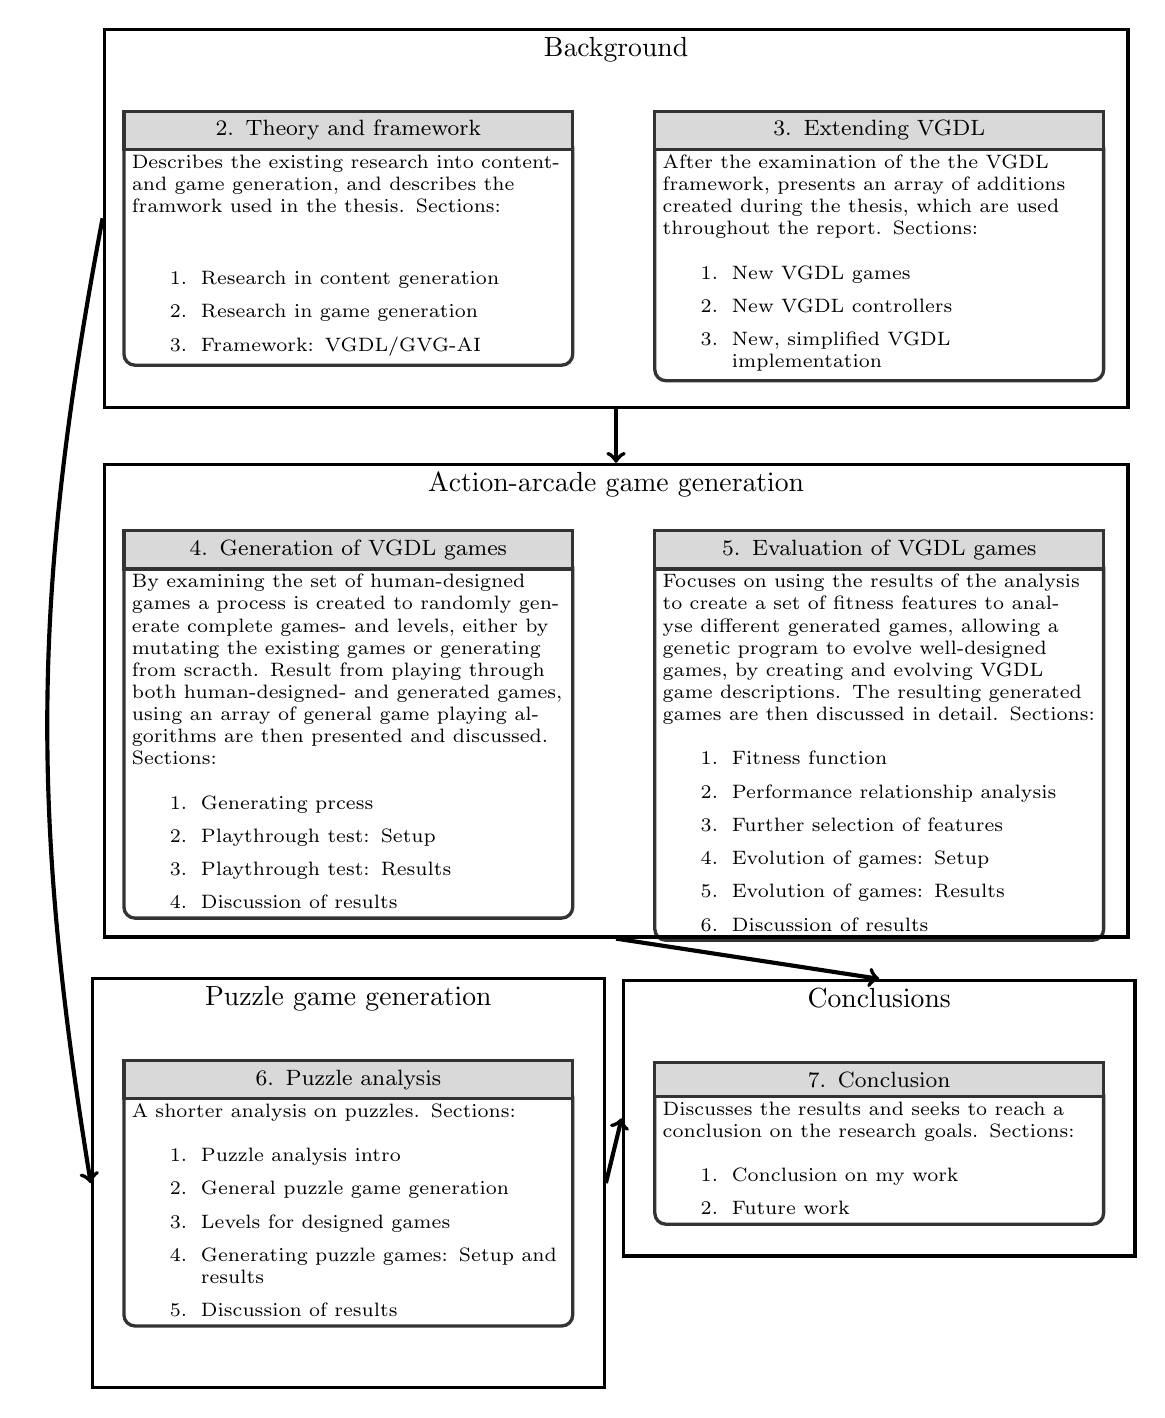
\begin{tikzpicture}[
chapterparts/.style={rectangle, draw=black!80, very thick, text width=5.5cm, font = \scriptsize,inner xsep = 0.1cm,rounded corners, align=left},
chapterheader/.style={rectangle, draw=black!80, fill=black!15, very thick, text centered, text width=5.5cm, font = \footnotesize,inner xsep = 0.1cm,},
largebox/.style={rectangle, draw=black, very thick, minimum size=7mm},
squarednode/.style={rectangle, draw=red!60, fill=red!5, very thick, minimum size=5mm},
nodes = {align = center}
]
%Nodes
\node[chapterheader]   (theoryh)		
{2. Theory and framework};
\node[chapterheader]   (backgroundh)  [right=of theoryh, shift = (right:0.0cm)]		
{3. Extending VGDL};
\node[chapterheader]   (task1h)  [below=of theoryh, shift = (down:3.8cm)]		
{4. Generation of VGDL games};
\node[chapterheader]   (task2h)  [right=of task1h, shift = (right:0.0cm)]		
{5. Evaluation of VGDL games};
\node[chapterheader]   (task3h)  [below=of task1h, shift = (down:5.2cm)]		
{6. Puzzle analysis};
\node[chapterheader]   (conclusionh)  [right=of task3h, shift = (right:0.0cm)]		
{7. Conclusion};
 % \begin{scope}[on background layer]
 \begin{pgfonlayer}{background}
\node[chapterparts]      (theory) [below=of theoryh, shift = (up:1.2cm)]	
									{\quad\\
									Describes the existing research into content- and game generation, and describes the framwork used in the thesis. Sections: \\\quad\\
									
									\begin{enumerate}\itemsep0pt
									\item Research in content generation
									\item Research in game generation
									\item Framework: VGDL/GVG-AI
									\end{enumerate}
									};
\node[chapterparts]      (background) [below=of backgroundh, shift = (up:1.2cm)]	
									 {\quad\\
									 After the examination of the the VGDL framework, presents an array of additions created during the thesis, which are used throughout the report. Sections:	
									 \begin{enumerate} \itemsep0pt
									\item New VGDL games
									\item New VGDL controllers
									\item New, simplified VGDL implementation
									\end{enumerate}
									};
\node[chapterparts]      (task1) [below=of task1h, shift = (up:1.2cm)]	
									 {\quad\\
									By examining the set of human-designed games a process is created to randomly generate complete games- and levels, either by mutating the existing games or generating from scracth. Result from playing through both human-designed- and generated games, using an array of general game playing algorithms are then presented and discussed. Sections:											 													\begin{enumerate}\itemsep0pt
									\item Generating prcess
									\item Playthrough test: Setup
									\item Playthrough test: Results
									\item Discussion of results
									\end{enumerate}
									};
\node[chapterparts]      (task2)[below=of task2h, shift = (up:1.2cm)]	
									 {\quad\\
									 Focuses on using the results of the analysis to create a set of fitness features to analyse different generated games, allowing a genetic program to evolve well-designed games, by creating and evolving VGDL game descriptions.
The resulting generated games are then discussed in detail. Sections:
									 \begin{enumerate}\itemsep0pt
									\item Fitness function
									\item Performance relationship analysis
									\item Further selection of features
									\item Evolution of games: Setup
									\item Evolution of games: Results
									\item Discussion of results
									\end{enumerate}
									};
\node[chapterparts]      (task3)[below=of task3h, shift = (up:1.2cm)]	
									 {\quad\\
									 A shorter analysis on puzzles. Sections:
									 \begin{enumerate}\itemsep0pt
									\item Puzzle analysis intro
									\item General puzzle game generation
									\item Levels for designed games
									\item Generating puzzle games: Setup and results
									\item Discussion of results
									\end{enumerate}
									};
\node[chapterparts]      (conclusion)[below=of conclusionh, shift = (up:1.2cm)]	
									 {\quad\\
									 Discusses the results and seeks to reach a conclusion on the research goals. Sections:											 													\begin{enumerate}\itemsep0pt
									\item Conclusion on my work
									\item Future work
									\end{enumerate}};
\node[largebox]			(backgroundbox)[above=of theoryh, shift = (down:4.8cm), shift = (right:3.4cm), minimum height = 4.8cm, minimum width = 13cm, label={[anchor=north]above:Background}]{};
\node[largebox]			(actionbox)[above=of task1h, shift = (down:6.2cm), shift = (right:3.4cm), minimum height = 6.0cm, minimum width = 13cm, label={[anchor=north]above:Action-arcade game generation}]{};
\node[largebox]			(puzzlebox)[above=of task3h, shift = (down:5.2cm), shift = (right:0.0cm), minimum height = 5.2cm, minimum width = 6.5cm, label={[anchor=north]above:Puzzle game generation}]{};
\node[largebox]			(conclusionbox)[above=of conclusionh, shift = (down:3.5cm), shift = (right:0.0cm), minimum height = 3.5cm, minimum width = 6.5cm, label={[anchor=north]above:Conclusions}]{};
\end{pgfonlayer}
%\end{scope}

%Lines
\draw[->,line width=1.5pt] (backgroundbox.south) -- (actionbox.north);
\draw[->,line width=1.5pt] (backgroundbox.west) to[bend right=10] (puzzlebox.west);
\draw[->,line width=1.5pt] (actionbox.south) -- (conclusionbox.north);
\draw[->,line width=1.5pt] (puzzlebox.east) -- (conclusionbox.west);
%\draw[->,line width=1.5pt] (theory.east) -- (background.west);
%\draw[->,line width=1.5pt] (theory.south) -- (task1h.north);
%\draw[->,line width=1.5pt] (theory.south) -- (task2h.north);
%\draw[->,line width=1.5pt] (background.south) -- (task1h.north); %to[bend left=10]
%\draw[->,line width=1.5pt] (theory.east) -- (task2.west)
%\draw[->,line width=1.5pt] (task1.south) -- (task3h.north);
%\draw[->,line width=1.5pt] (theory.west) to[bend right=20] (task3.west);
%\draw[->,line width=1.5pt] (background.west) -- (task3.east);
%\draw[->,line width=1.5pt] (task1.east) -- (task2.west);
%\draw[->,line width=1.5pt] (task2.south) -- (conclusionh.north);
%\draw[->,line width=1.5pt] (task3.south) to[bend right=45] (conclusion.south);

\end{tikzpicture}
%\end{center}
\caption{How to read this thesis}
\label{fig:vgdlgame}
\end{figure}


%------------------------------------------------------------------------------------------------------------------------------%
%------------------------------------------------------------------------------------------------------------------------------%
%------------------------------------------------------------------------------------------------------------------------------%
\chapter{Existing research and framework}
\label{ch_existingresearch}
In this chapter I describe the existing research on the topic of procedural content generation (PCG) for games, and specifically game- and level-generation, which is of relevance to the project.
Additionally the framework used for game- and level-generation, and testing is described thoroughly.



\section{Content generation}
\label{sec_contengen}
%Before discussing generation of complete games, the research on procedural content generation (PCG) for games is  discussed. 
The task of PCG is to create elements for specific parts of a game, for instance levels, weapons, environments, textures and sounds. 
%\citet{hendrikx2013procedural} proposes a layered taxonomy to describe PCG of different depths in games, while performing a survey of different ways in which PCG has been implemented in commercial games, noticing that some layers has not been thoroughly explored.

Several different approaches are used in PCG (both in commercial games and in research), however the ``search-based'' approach (explored by \citet{togelius11search}, \citet{pcgbook:ch2}) dominates the problem.
In search-based generation a \textit{fitness function} is used to score generated content by their quality, making it possible to ensure a high quality of the generator, by either simply generating a large amount of content and choosing the best, or using an evolutionary strategy to evolve better content.




%\subsubsection*{Game-level generation}
%Almost all video games are highly dependent on a set of levels or maps, in which the game play takes place. Levels are often responsible for creating increasingly challenging situations, and thereby entertaining game play. 
%Super Mario would be way less interesting if enemies and platforms were spread randomly across each level, which would almost certainly result in the game being ether too easy or too difficult.
%Several scientific projects have focused on the topic of level-generation with an array of different approaches, some requiring player-input, or simply a helper for human level-designer.

%In addition to the other game genres mentioned above, a lot of work has been done in generating levels for puzzle games (ie. Sokoban and Cut The Rope).
%Most of the work is focused on generating levels for single game, where some attempt to create general level generation procedures.


%\subsection{Other uses of PCG}
%Other games have been published applying PCG in different ways. In \textit{Borderlands 2} \citeyearpar{game:borderlands} the player have access to an extreme amount of different weapons, designed by automatic generation.


%\subsubsection*{Advantages and disadvantages using PCG}
%
%Having a procedure for generating content in games has a number of advantages:
%
%\begin{itemize}
%  \item Content generation allows games to potentially have an endless amount of possibilities, often resulting in higher re-play value than linear games. 
%  \item PCG can help game designers generate game levels, often simply by letting the designer explore possible layouts, add decorations or finishing up human-designed levels.
%\end{itemize}
%
%PCG also has some problems for generating content for levels:
%
%\begin{itemize}
%  \item Generated content can have a feeling of being unauthentic and/or too random. For instance, the positions of decorations in a level (barrels, paintings etc.) can be important for humans, while they are not for computers.
%  \item In games where the player follows a story it can be difficult to automatically generate levels, that follow what the game designer intend to happen%.
%\end{itemize}




\section{Game generation}
\label{sec_gamegen}
Generating complete games through algorithms is a problem that is being increasingly researched, but progress on the topic for last decade. Because the problem is in general quite large, a subset of the problem is usually handled: Only generating certain types of games-, or using different (restricted) frameworks. 
Video games may consist of a large number of tangible and intangible components, including rules, graphical assets, genre conventions, cultural context, controllers, character design, story and dialog, screen-based information displays, and so on~\citet{cook2014angelina,liapis2014creativity,nelson2007automated}.

In this project I look specifically at generating the game-play and -setting of games, i.e. defining a set of game-rules and -objects, and specifying the levels in which the game-play takes place.
The two main approaches that have been explored in generating game rules are reasoning through constraint solving~\citet{smith2010variations} or search through evolutionary computation or similar forms of stochastic optimisation~\citet{togelius2008experiment,browne2008automated,font2013towards}. 
In either case, rule generation can be seen as a particular kind of procedural content generation~\citet{pcgbook:ch6}.

%The idea of generating complete games through algorithms is not itself new. The problem in full generality is quite large, so usually a subset of the general problem is tackled. Videogames may be comprised of a large number of tangible and intangible components, including rules, graphical assets, genre conventions, cultural context, controllers, character design, story and dialog, screen-based information displays, and so on~\citet{cook2014angelina,liapis2014creativity,nelson2007automated}.

%In this paper I look specifically at generating game rules; and more specifically the rules of arcade-style games based on graphical movement and local interaction between game elements, represented in the game description language VGDL. The two main approaches that have been explored in generating game rules are reasoning through constraint solving~\citet{smith2010variations} or search through evolutionary computation or similar forms of stochastic optimisation~\citet{togelius2008experiment,browne2008automated,font2013towards}. In either case, rule generation can be seen as a particular kind of procedural content generation~\citet{pcgbook:ch6}.

It is clear that generating a set of rules that makes for an interesting and fun game is a hard task. 
The arguably most successful attempt so far, Browne's Ludi system, managed to produce a new board game of sufficient quality to be sold as a boxed product~\citet{browne2008automated}. 
However, it succeeded partly due to restricting its generation domain to only the rules of a rather tightly constrained space of board games. 
A key stumbling block for search-based approaches to game generation is the fitness/evaluation function. 
This function takes a complete game as input and outputs an estimate of its quality. Ludi uses a mixture of several measures based on automatic playthrough of games, including balance, drawishness and outcome uncertainy.
These measures are well-chosen for two-player board games, but might not transfer that well to video games or single-player games, which have in a separate analysis been deemed to be good targets for game generation~\citet{togelius2014characteristics}. 
Other researchers have attempted evaluation functions based on the learnability of the game by an algorithm~\citet{togelius2008experiment} or an earlier and more primitive version of the characteristic that is explored in this paper, performance profile of a set of algorithms~\citet{font2013towards}.

A typical approach for generating complete games is searching in a space of possible games. This basically requires two things: That the ratio of enjoyable games in the set is not too low - otherwise those games might never be found. To increase this ratio a game description language (GDL) is often used (searching through all possible Java or C programs would lead to an enormous amount invalid games).
Also, to search through a set of games it is necessary to be able to calculate a fitness value for each game, valuing how enjoyable the game is.


%\subsection{Something to note: Levels}
%\label{ssec_notelevels}
%The problem of generating complete games is heavily linked to the problem of generating levels since most games are deeply tied to the geometry and object-placement defined in levels.
%A part of the success of Ludi stem from the fact that levels (boards) were as much in focus, as the game-rules themselves.





\section{Framework: VGDL and the GVG-AI framework}
\label{sec_gvgaiframework}
Regardless of which approach to game generation is chosen, one needs a way to represent the games that are being created. %\footnote{See \citet{pcgbook:ch6} for a discussion of game-rule representation choices.} 
For a sufficiently general description of games, it stands to reason that the games are represented in a reasonably generic language, where every syntactically valid game description can be loaded into a specialised game engine and executed. 
There have been several attempts to design such GDLs. One of the more well-known is the Stanford GDL, which is used for the General Game Playing Competition~\citep{genesereth2005general}. The language is tailored to describing board games and similar discrete, turn-based games. 
However, it is arguably too verbose and low-level to support search-based game generation. 
Another attempt at an VGDL is called PuzzleScript \citep{puzzlescript}, created by game designer Stephen Lavelle. 
The language -- as its name suggest -- is focused on (turn-based) puzzle games, but the engine allows for simple forms of animation and movement, for a more action-oriented game design. 
The language is relatively high level compared to Stanford GDL, but at as result the complete space of  games is rather restricted.


\subsection{VGDL game descriptions}
\label{ssec_vgdl}
The various game generation attempts discussed above feature their own GDLs of different levels of sophistication; however, there has not until recently been a GDL for suitably for a larger space of video game types- and genres.
The Video Game Description Language (VGDL) is a GDL designed to express 2D arcade-style video games of the type common on hardware such as the Atari 2600 and Commodore 64. 
It can express a large variety of games in which the player controls a single moving avatar (player character) and where the rules primarily define what happens when objects interact with each other in a two-dimensional space. 
VGDL was designed by a set of researchers~\citet{levine2013general,ebner2013towards} (and implemented by Schaul ~\citet{schaul2013video}) in order to support both general video game playing and video game generation.
In contrast to other GDLs, the language has an internal set of classes, properties and types that each object can defined by, which the authors suggest the user to extend.

Objects have physical properties (i.e. position, direction) which can be altered either by the properties defined, or by interactions defined between specific objects. 
Playing the games also required a specified level which defines a set of game tiles, indicating the initial locations of sprites. 
Each sprite can move a distance specified by its \texttt{speed}-parameter in the four cardinal direction, which supports decimal values causing sprites to be able to move in-between game tiles.

A VGDL description has four parts: 


\subsubsection*{SpriteSet}
Defines which sprites can appear in the game. Each sprite must be designated by a class, in which a set of predefined actions exists. Also a set of parameters can (and sometimes, must) be fed to each sprite, configuring for instance the \texttt{speed} or how often the sprite takes an action -- using the \texttt{cooldown}-parameter -- and a set of parameters unique to the different sprite-classes.
For instance, for the  class \texttt{Flicker}\footnote{\texttt{Flicker}s is a simple extension to the base sprite; the sprite is destroyed after a speecifed amount of time.} the lifetime can be adjusted, and the \texttt{Chaser} sprite class\footnote{\texttt{Chaser} sprites move towards a specified other sprite, every time it is allowed to move.} it is necessary to define which object to actually chase.
Another interesting sprite types is the \texttt{Resource}-class, which, in combination with interaction-rules, can be ``collected'' by other sprites and several effects can occur (again defined in the interaction-rules), like ``if avatar has collected more than 10 coins, he/she is killed when touching wall sprites''.
Sprites can additionally be designed in a tree structure, where multiple sprites have the same parent sprite, making descriptions for interaction- and termination rules (described below) less verbose. 

\subsubsection*{InteractionSet}
Each line of the \texttt{InteractionSet} specifies a pair of sprites and an effect, defining the resulting effect of the two sprites interacting with each other (i.e. colliding with each other).
Possible interaction effects include \texttt{stepBack}, causing the first sprite specified to be pushed back to its last position, \texttt{bounceForward}, causing the sprite to be pushed one tile forward, and \texttt{killSprite}, which simply kills the first sprite defined on collision.
Many interaction effects additionally have parameters which must be set for the rules to have a function, for instance for the rule \texttt{transformTo} (which converts the first sprite defined from one type to another), it must be defined which sprite to transform to.
All interaction effects also have a possibility of changing the players score on collisions.


\subsubsection*{TerminationSet}
The termination set defines how the game can end. 
Each line in this set has a win parameter, which is set to true or false; determining if the effect causes a winning or losing the game.
Each termination-function is represented by a class defining under which conditions the game should end, for instance the \texttt{SpriteCounter} class can cause the game to be won or lost, when there exists 0 of a certain sprite  (when all of the sprites are killed).
Most of the VGDL games examined- and generated in this thesis simply contain two termination rules: 
A win- and a lose- termination.

\subsubsection*{LevelMapping}
The job of the \texttt{LevelMapping} (see figure \ref{fig:vgdlgame_level}) is to translate from a character (\texttt{char}) in a level-file (explained below), to sprites from the \texttt{SpriteSet}. 
A single mapping can be shared by several sprites, causing a series of sprites to be created on the same game-tile.




\begin{figure}[!ht]
\centering
\begin{vgdldesc}[linewidth=14cm]
BasicGame
    SpriteSet
        forestDense > SpawnPoint stype=log prob=0.4  cooldown=10 img=forest
        forestSparse > SpawnPoint stype=log prob=0.1  cooldown=5 img=forest
        structure > Immovable
            water > color=BLUE img=water
            goal  > Door color=GREEN img=goal
        log    > Missile   orientation=LEFT  speed=0.1 color=BROWN img=log
        safety > Resource  limit=2 color=BROWN img=mana
        truck  > img=truck
            rightTruck  > Missile   orientation=RIGHT 
                fastRtruck  > speed=0.2  color=ORANGE
                slowRtruck  > speed=0.1  color=RED
            leftTruck  > Missile   orientation=LEFT
                fastLtruck  > speed=0.2  color=ORANGE
                slowLtruck  > speed=0.1  color=RED
        # defining 'wall' last, makes the walls show on top of all other sprites
        wall > Immovable color=BLACK img=wall
        
    InteractionSet
        goal avatar  > killSprite scoreChange=1
        avatar log   > changeResource resource=safety value=2
        avatar log   > pullWithIt   # note how one collision can have multiple effects
        avatar wall  > stepBack
        avatar water > killIfHasLess  resource=safety limit=0
        avatar water > changeResource resource=safety value=-1
        avatar truck > killSprite scoreChange=-2
        log    EOS   > killSprite
        truck  EOS   > wrapAround
    
    TerminationSet
        SpriteCounter stype=goal   limit=0 win=True
        SpriteCounter stype=avatar limit=0 win=False
    
    LevelMapping
        G > goal
        0 > water
        1 > forestDense water       # note how a single character can spawn multiple sprites
        2 > forestDense wall log
        3 > forestSparse water       # note how a single character can spawn multiple sprites
        4 > forestSparse wall log
        - > slowRtruck
        x > fastRtruck
        _ > slowLtruck
        X > fastLtruck
        = > log water
        B > avatar log
\end{vgdldesc}
\caption{Example of a VGDL game description: An interpretation of the classic arcade game \textit{Frogger}}
\label{fig:vgdlgame}
\end{figure}

\subsubsection*{Level description}
Besides the four sets used to describe a game in VGDL, to actually play a game a level file is additionally needed, defining the initial positions of a set of sprites using the \texttt{SpriteSet} combined with the \texttt{LevelMapping}, in which each textual character defines which sprites to appear in which tile-, while spaces defines empty tiles of the game.

\begin{figure}[!ht]
\centering
\begin{vgdldesc}[linewidth=14cm]
wwwwwwwwwwwwwwwwwwwwwwwwwwww
w           wGw            w
w00==000000===0000=====000=2
w0000====0000000000====00012
w00===000===000====0000===02
www   ww   www    www  wwwww
w   ----   ---   -  ----   w
w-     xxx       xxx    xx w
w -   ---     -   ---- --  w
w       A                  w
wwwwwwwwwwwwwwwwwwwwwwwwwwww
\end{vgdldesc}
\caption{Example of a VGDL level description: A level for the interpretation of \textit{Frogger}}
\label{fig:vgdlgame_level}
\end{figure}



\subsection{The GVG-AI framework: AI controllers and testing}
\label{ssec:aicontrollersandtesting}
The GVG-AI framework is a testbed for testing general game-playing controllers on games specified using VGDL. 
Controllers are called once at the beginning of each game for setup, and then once per clock tick to select an action. 
Controllers do not have access to the VGDL descriptions of the games. They receive only the game's current state; the position of each sprite, and their ``types'' (e.g. portal, immovable, resource), passed to a controller when it is asked to select an action. 
However these states can importantly be forward-simulated to future states. 
Thus the game rules are not directly available, but a simulatable model of the game can be used.

\subsubsection*{GVG-AI sample controllers}
A series of general game playing controllers is additionally available in the framework, using a series of different approaches to select an action on each clock tick.
One of these controllers were chosen to be used in this project to examine designed- and generated games:

\begin{description}
	\item [SampleMCTS] Simulates the game space of possible actions within a small area of the games, using a open-loop search and a ``Vanilla'' MCTS approach using UCT.
%	\item [GA] Uses a genetic algorithm to evolve a sequence of actions.
%	\item [OneStep-Heuristic] Heuristically evaluates the states reachable through one-step lookahead. The heuristic takes into account the locations of NPCs and certain other objects.
\end{description}

\subsubsection*{GVG-AI example games}
The framework additionally contains 20 human-designed games, which partly consist of interpretations of classic video games (e.g. Boulderdash, Frogger, Missile Command and Pacman), while some are original creations by the General Video-Game AI Competition's organisers. 
The interpretations of existing games all have different stages of simplifications to them, causing several of the games' features to be missing -- for instance, the player cannot push boulders in the VGDL version of Boulderdash and they do not ``roll'' as in the original, and the ghosts in Pacman behave in a much more simplified fashion than in the original.
A short summary of each of the example games can be seen in Appendix \ref{app_gvgaigames}

The games are -- except for the game \emph{Sokoban} -- of the \textit{action-arcade} genre (defined in the introduction), in that the player controls a single avatar which must be moved quickly around in a 2D-setting to win, and to get a high score.
Figure \ref{fig:vgdlgame} shows the VGDL description of the game \emph{Frogger}, and \ref{fig:vgdlgame_level} a level description from the same game.
Figure \ref{fig:gvgai_games_screenshots} show how some of the games are visually represented when playing in the GVG-AI framework.


\begin{figure}[!ht]
	\subfloat{
      		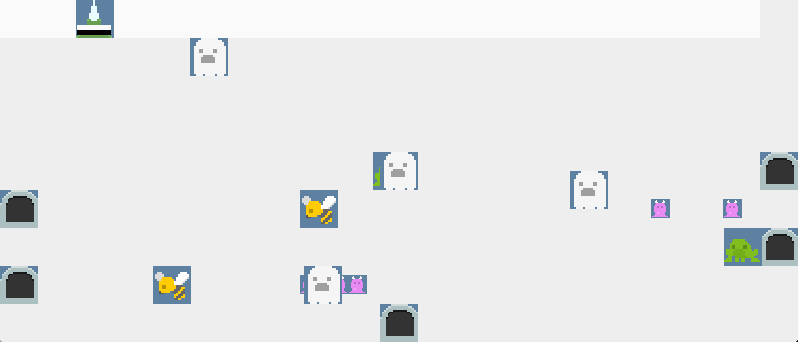
\includegraphics[scale=0.3]{seaquest.png}
    	}
	\hfill
	\subfloat{
      		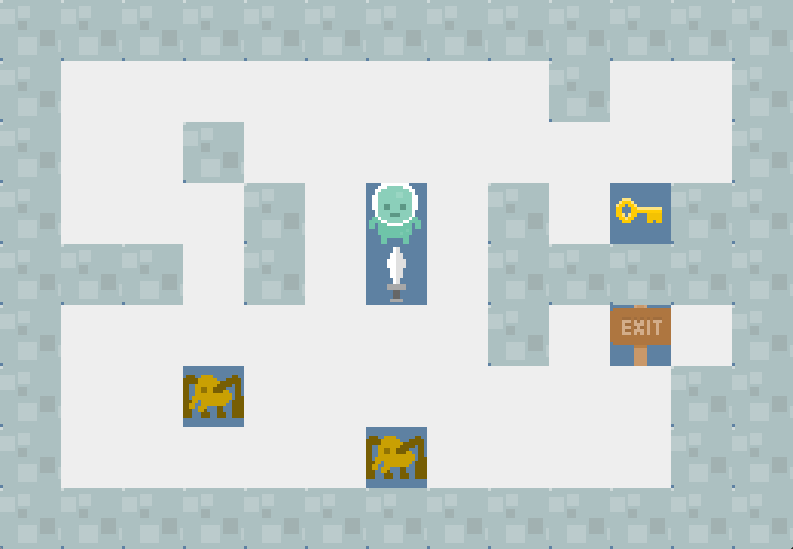
\includegraphics[scale=0.19]{zelda.png}
    	}\\
	\subfloat{
		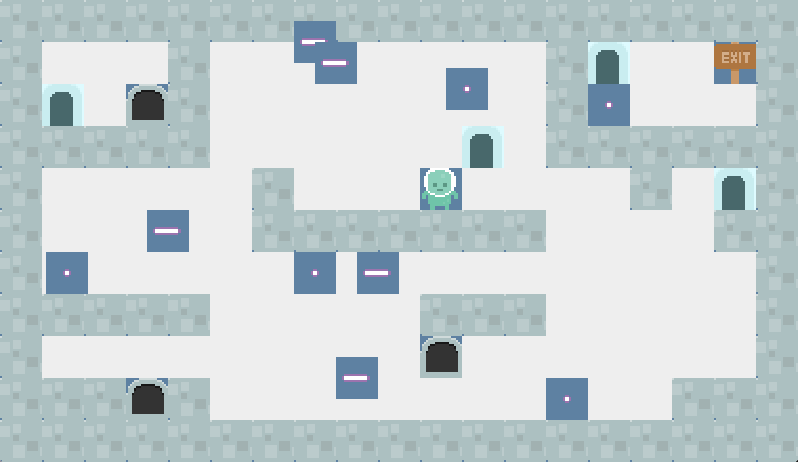
\includegraphics[scale=0.24]{portals.png}
	}\hfill
	\subfloat{
      		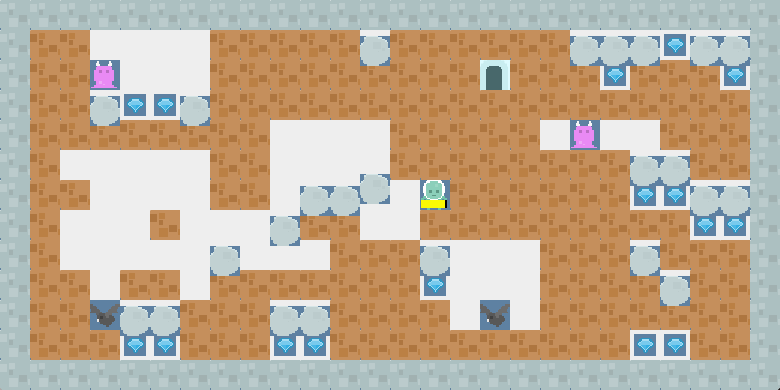
\includegraphics[scale=0.29]{boulderdash.png}
    	}\\
	\subfloat{
      		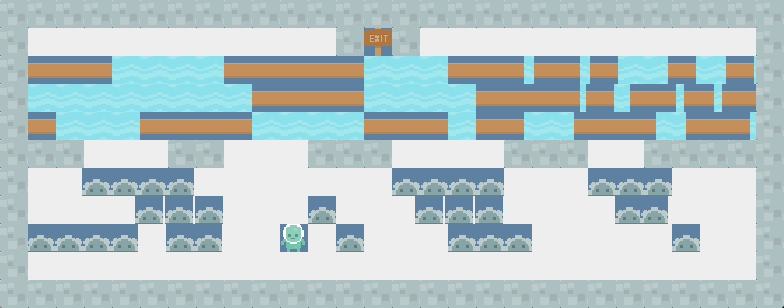
\includegraphics[width=\textwidth]{frogs.png}
    	}\\
    	\caption{The visual representation of a few of the VGDL example games which are interpretations of commercial games. From top-left: \textit{Seaquest}, \emph{Zelda}, \emph{Portals}, \emph{Boulderdash} and \textit{Frogs} (\textit{Frogger}).}
	\label{fig:gvgai_games_screenshots}
\end{figure}





\subsubsection*{Game genres of VGDL and the GVG-AI framework}
\label{ssec_gamegenres}
Using the VGDL implementation of the GVG-AI framework the games that can be described are rather restricted to certain genres- and types, without greatly extending the program.
For instance, the lack of possibility to traverse different levels in the same play through make \textit{adventure} games unattainable, and the restriction of only moving a single character with the keyboard (the avatar) makes great restriction in creating \textit{strategy} games.

The games examined- and generated in this thesis are of a type that makes them suitable for the framework: Action-arcade- and puzzle games. 

As mentioned in the introduction,  I make the simple distinction between the two types of games in the VGDL framework, that arcade games can contain elements (sprites) that move by themselves, whereas interactions only occur as a result of the avatar moving in puzzle games.
As a results, certain sprites- and interaction classes are restricted to the action-arcade games (e.g. NPC- and Missile sprites), making the space of possible VGDL \textit{puzzle games} slightly smaller.


%------------------------------------------------------------------------------------------------------------------------------%
%------------------------------------------------------------------------------------------------------------------------------%
%------------------------------------------------------------------------------------------------------------------------------%

\chapter{Extending VGDL}
\label{ch_extending}
This chapter describes a series of extensions I constructed for the GVG-AI framework, making a more in-depth analysis possible.
I created a series of VGDL games, AI controllers and a implemented a new, simplified framework to play through \textit{puzzle games} with less time and memory use.


\section{Writing new VGDL games}
\label{sec_writingnewvgdl}
To increase the size of the set of designed games, to allow for a more precise analysis of what makes a good game, I created fourteen new game descriptions in VGDL. 

Another important reason for creating new descriptions, was to introduce a series of \emph{puzzle games} to be analysed, since, as mentioned in Section \ref{ssec_vgdl} the example games from the GVG-AI competetion are almost all of the \textit{action-arcade} genre.


\subsubsection*{Describing existing games in VGDL}
The main goal when developing a game - which also applies in this case - is to ensure that it is enjoyable to human-players. 
Therefore the games implemented are all interpretations of published existing games (and not original creations).
As described in Section \ref{ssec_gamegenres} VGDL can only describe relatively simple games of certain types/genres, and so only a limited number of games can be translated without severely changing the gameplay.

The games I created (described below) are in general ``true'' copies of the originals - containing all the gameplay features and interactions but lacking elements like audio, graphics and controls. 
However many lack certain (non-essential) game-play features like bonus points (like fruits in Pac-Man), infrequently appearing enemies (UFOs in Space Invaders) or features which only appear in later levels of the games.


\subsubsection*{Interpreted games}
A series of fourteen commercial games was re-created in VGDL to be used in future tests. 
Figure \ref{fig:centipedeTranslation} shows one of the games translated to VGDL.
Minor changes to the GVG-AI framework was made for a small number of the games, to be able to correctly copy the games' core gameplay features.
The original game levels were additionally translated into VGDL level description, with five levels being created for each game.
For some of the games the levels could not be completely copied, for instance because the levels were too large in size (\textit{Bolo Adventures}), or because a lack of game features implemented in the clones (\textit{Chip's Challenge}), and the resulting levels are therefore simplifications of the originals..

\subsubsection*{Action-arcade games}
A set of four Atari -arcade and -2600 games were found to be suitable for interpretation; \textit{Solar Fox}, \textit{Crackpots}, \textit{Centipede} and \textit{Astrosmash}, and a VGDL game description was written for each. 
A description of each of the games and their interpretations can be seen in Appendix \ref{app_thesisgames}.

\begin{figure}[!ht]
${\vcenter{\hbox{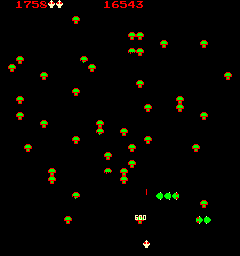
\includegraphics[height=6cm]{origcentipede.png}}}} \vcenter{\hbox{\scalebox{2}{\Huge\pointer}}}
\vcenter{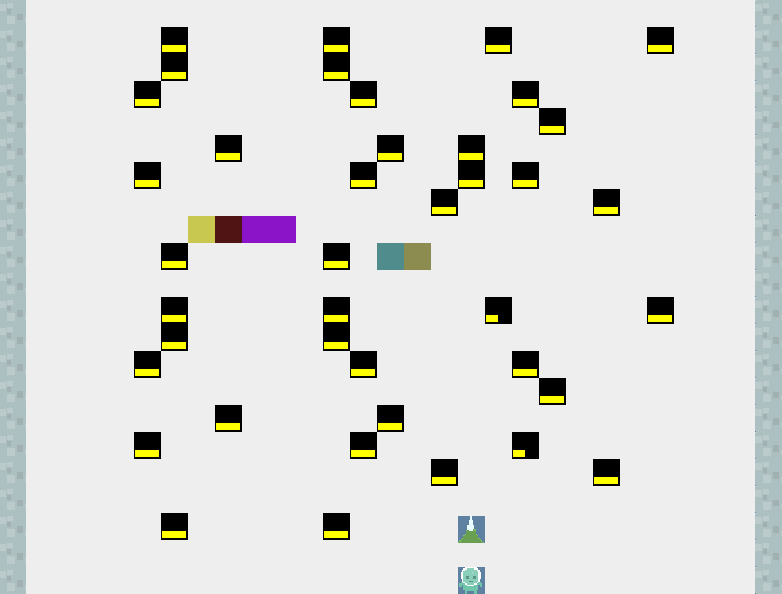
\includegraphics[height=6cm]{vgdlcentipede.png}}
$
    	\caption{Interpretation of the classic arcade game \textit{Centipede} \citeyearpar{game:crackpots}}
\label{fig:centipedeTranslation}
\end{figure}


\subsubsection*{Puzzle games}
A set of puzzle games from several different platform, all featuring a single avatar, was found to be suitable to be described in VGDL. 
The games can mostly be described as \textit{Sokoban}-clones with different spins on the gameplay.
Some of the games have action- gameplay aspects, with enemies hindering the progression of the player, but as per the defintion of \textit{puzzle games} used in the thesis these parts were removed only leaving the puzzles of games.

However, even with the removal of enemies, a few of the interpreted games contain elements which are not strictly in line with the definition of VGDL \textit{puzzle games}, for instance some of games feature gliding boxes or rolling boulders (implemented using the \texttt{Missile} sprite class), which can cause effects to happen many frames after the avatar has acted.

The games interpreted were \textit{Sokoban}, \textit{Bait}, \textit{Bombuzal}, \textit{Bolo Adventures}, \textit{Zen Puzzle}, \textit{The Citadel}, \textit{Brainman}, \textit{Chip's Challenge}, \textit{Modality} and \textit{Painter}.
A summary of the games can be seen in Appendix \ref{app_thesisgames}.

\begin{figure}[!ht]
${\vcenter{\hbox{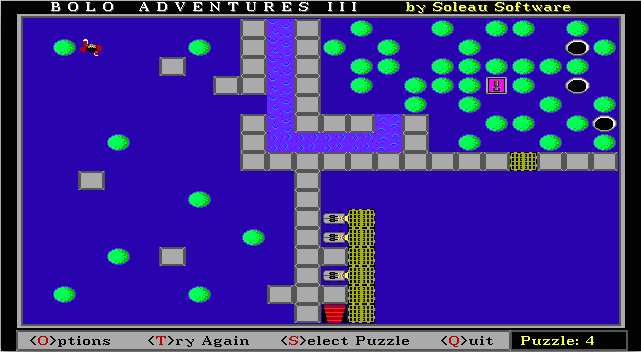
\includegraphics[height=4.8cm]{origboloadventures.png}}}} \vcenter{\hbox{\scalebox{2}{\Huge\pointer}}}
\vcenter{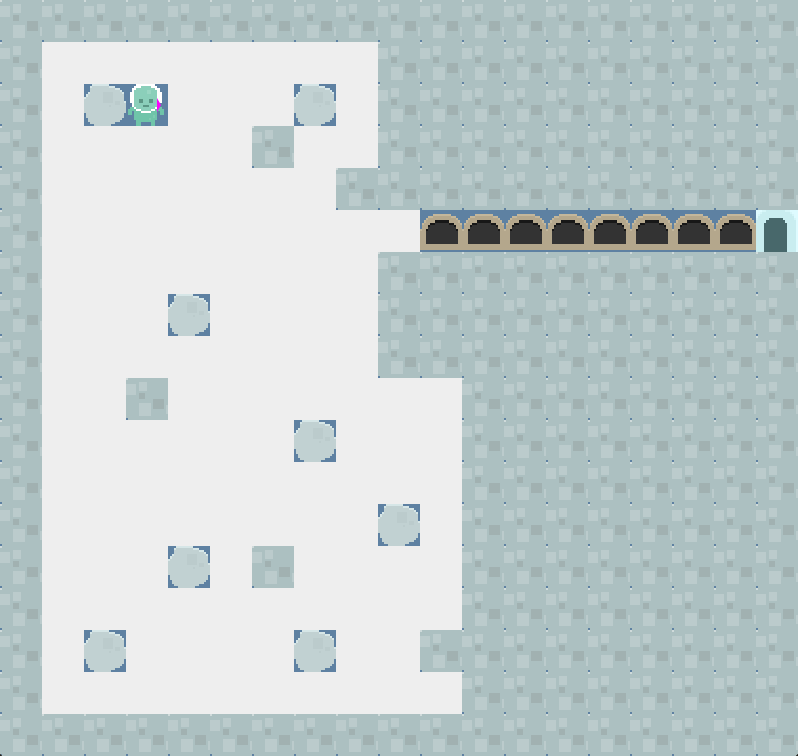
\includegraphics[height=4.8cm]{vgdlboloadventures.png}}
$
    	\caption{Interpretation of both the game and part of a level, from the DOS game Bolo Adventures III}
\label{fig:centipedeTranslation}
\end{figure}




%------------------------------------------------------------------------------------------------------------------------------%

\section{Creating new VGDL controllers}
\label{sec_creatingnewcontrollers}
To be able to probe VGDL games in more detail, I created a series of new AI controllers with various approaches to finding the action to take.
In total four new controllers was generated: Three to play the action-arcade style games, and one only focused on solving puzzle games.

\subsubsection*{Action-arcade controllers}
Three controllers of an increasing degree of cleverness was introduced: \textit{One-step} (simplest), \textit{Deep-search} and \textit{Explorer} (most complex), with different strategies used in simulating the forward model (accessible when running the GVG-AI framework).
% exploring the game space with different series of actions.


\begin{description}
\item[OneStep] The One-step algorithm only attempts to advance the forward model once for each allowed action in the game.
The score and win/lose state of the resulting game states are then considered, and the action with the resulting best state is chosen, with a random action chosen when no state is better than others.
The controllers approach can be seen below:

\begin{algorithm}[H]
\For{action : PossibleActions}{
newGameState = gameState.copy().advance(action) \\
value[action] = value(newGameState) \\
}
\Return action leading to highest value, or random action if values are equal
\caption{One-step algorithm}
\end{algorithm}

\item[DeepSearch]
This controller starts out in a similar fashion as the One-step, by expanding using all possible actions by copying the initial game-state.
These game-states are then simulated further upon by advancing each game state a single time, with a partly\footnote{A key part of success of the algorithm is that it, after the initial expansion, never tries to advance in a opposite movement direction to the initial.} random action, without copying the state (which is a rather costly procedure).
This expansion is continued until the controller runs out of time, and a value for each action is calculated by considering the score and win/lose-value for each state that can be achieved from each of the initial states. \\

\begin{algorithm}[H]
queue $\gets$ initial gameState \\
\While{has time left}{
	gameState = queue.poll() \\
	\eIf{gameState == initial gameState}{
		\For{action : PossibleActions}{
			queue $\gets$ gameState.copy().advance(action)
		}
	}{
		gameState.advance(random action) \\
		d $\gets$ depth of search //amount actions performed \\
		value[action] $+=$ value(newGameState) $* \text{PossibleActions.length}^{\text{d}}$
	}
}
\Return action leading to highest value, or random action if values are equal
\caption{Deep-search algorithm}
\end{algorithm}

\item[Explorer]
The explorer controller was designed specifically to play the arcade-style games of the GVG-AI framework, and utilizes a series of methods to strengthen its decisions. 
Unlike the other controllers which utilise open-loop searches, it stores information about visited tiles and prefers visiting unvisited locations. 
In addition the controller uses three different arrays to choose an action on each clock tick: 
1) One considering how probable death is from each action, 2) one examining the score that can be achieved from the actions, and 3) one only looking at the boringness -- which changes dependant on which tiles has been visited.
If the \textit{death}-array have too high values, that array is used to take the decision (the action leading to the lowest value is chosen), otherwise the best action from the score-array is used.
If the values of the \textit{score}-array happen to be too similar, the boringness-array is used as last resort.

The controller also addresses a common element of the VGDL example games, randomness. The controller gains an advantage in many of the games by simulating the results of actions repeatedly, before deciding the best action.

The Explorer was proven to be of a decent quality by getting a 1st / 5th place in the GVG-AI's competition between controllers \footnote{The controller (nicknamed \textit{thorbjrn_other}) has at the time of writing (28/02-2015) a 1st place in the training set of the competition (first 10 games of the GVG-AI framework), and 5th in the validation set (the second 10 games): http://gvgai.net/gvg_rankings.php?rg=1}.
\end{description}



\subsubsection*{Puzzle controller}
The general game playing algorithms from the GVG-AI competition- and the algorithms described above are not well-suited for playing \emph{puzzle games}, because the goal can often only be achieved by applying a specific series of actions in the genre, which the controllers are not very good at.
To analyse an arbitrary puzzle game and be able to find the fastest solution, a breadth-first search algorithm was implemented, using a few methods to decrease the state-space by assumptions of the games.

\begin{description}
\item[PuzzleSolver]
The PuzzleSolver algorithm use the fact the puzzle games (using the definition of the introduction) only contain elements which can be moved or interacted with by the player-avatar, and contains no random elements, and so the initial state of a game in GVG-AI can be used to simulate all possible actions that eventually will lead to finding the solution of the games.
Additionally the PuzzleSolver uses the face that most of the puzzle games contain wall-sprites which always push back the player, and so the controllers never try to move into a wall -- this is achieved by storing the positions of every wall-sprite at the start of the game, and never simulating actions that lead to the avatar in a walls position.
\end{description}

Also, for each path the algorithm attempts, a signature of the game state is calculated and stored, constructed from the position and types of each (non-wall) sprite appearing in the given state. 
A path is cut off if the calculated game state is the same as has appeared before.

A problem of the approach is that controller adds several more signatures than needed if the game contains for instance \texttt{Missile}- or \texttt{Flicker} sprites, which are used in a few of the designed \textit{buzzle games}..
For the latter type of sprite a solution was implemented by ``skipping'' game states in which a \texttt{Flicker}-sprite exists (which have a limited lifetime), simply returning a NIL action until all \texttt{Flickers} has disappeared.
%To reduce the set of signatures needed to be stored, the algorithm additionally "skips" game states in which a \texttt{Flicker}-sprite exists (which have a limited lifetime), simply returning a NIL action until the \texttt{Flicker} has disappered.



%------------------------------------------------------------------------------------------------------------------------------%

\section{SimpleVGDL}
\label{sec_fastvgdl}
Since the GVG-AI framework has some functions and properties which are not important for, especially, the \textit{puzzle games} analysed in this work, I created an implementation of a lighter version of VGDL, solely focused on analysing puzzle games in more detail.
The implementation is basically a clone of the GVG-AI framework, but with several time- and memory consuming features removed, which in part was possible due to the puzzle games being relatively more simple (for instance, only movement from one tile to another is possible in SimpleVGDL, whereas sprites can move and collide in-between tiles in the GVG-AI framework).

In the SimpleVGDL framework the PuzzleSolver algorithm was additionally geared up with a two different approaches to memory handling: 1) Storing the actual game state for nodes in the search queue, and 2) only storing the game state signature and path, making it necessary to re-create the game state from the initial state of the game, whenever an element is polled from the queue.

Below I present the results of a small test of running a increasingly difficult game/level-pairs using the puzzle solver, in both the GVG-AI framework and using SimpleVGDL, both with- and without the ``low-memory'' option.

\begin{figure}[!ht]
\centering
\csvreader[tabular=lrrrrr,
    table head=\toprule \textit{\textbf{framework}}
             & \textit{time}
             & \textit{mem.},
    late after head=\csvifoddrow{\\\rowcolor{black!5}}{\\\rowcolor{black!25}}\midrule,
    late after line=\csvifoddrow{\\\rowcolor{black!5}}{\\\rowcolor{black!25}},
    late after last line=\\\bottomrule
    ]%
{fastvgdlsokoban3.csv}{1=\Framwork, 2=\Time, 3=\Space}%
{\Framwork & \Time & \Space}%
\caption{Results from playing through the game \textit{(Real) Sokoban}, level 4 (of 5) using the puzzle solver controller}
\label{table:fastvgdlsokoban3}
\end{figure}

 \begin{figure}[!ht]
\centering
\csvreader[tabular=lrrrrr,
    table head=\toprule \textit{\textbf{framework}}
             & \textit{time}
             & \textit{mem.},
    late after head=\csvifoddrow{\\\rowcolor{black!5}}{\\\rowcolor{black!25}}\midrule,
    late after line=\csvifoddrow{\\\rowcolor{black!5}}{\\\rowcolor{black!25}},
    late after last line=\\\bottomrule
    ]%
{fastvgdlsokoban1.csv}{1=\Framwork, 2=\Time, 3=\Space}%
{\Framwork & \Time & \Space}%
\caption{Results from playing through the game \textit{(Real) Sokoban}, level 2 (of 5) using the puzzle solver controller}\label{table:fastvgdlsokoban1}
\end{figure}

 \begin{figure}[!ht]
\centering
\csvreader[tabular=lrrrrr,
    table head=\toprule \textit{\textbf{framework}}
             & \textit{time}
             & \textit{mem.},
    late after head=\csvifoddrow{\\\rowcolor{black!5}}{\\\rowcolor{black!25}}\midrule,
    late after line=\csvifoddrow{\\\rowcolor{black!5}}{\\\rowcolor{black!25}},
    late after last line=\\\bottomrule
    ]%
{fastvgdlthecitadel4.csv}{1=\Framwork, 2=\Time, 3=\Space}%
{\Framwork & \Time & \Space}%
\caption{Results from playing through the game \textit{The Citade}, level 5 (of 5) using the puzzle solver controller}\label{table:fastvgdlthecitadel4}
\end{figure}

 \begin{figure}[!ht]
\centering
\csvreader[tabular=lrrrrr,
    table head=\toprule \textit{\textbf{framework}}
             & \textit{time}
             & \textit{mem.},
    late after head=\csvifoddrow{\\\rowcolor{black!5}}{\\\rowcolor{black!25}}\midrule,
    late after line=\csvifoddrow{\\\rowcolor{black!5}}{\\\rowcolor{black!25}},
    late after last line=\\\bottomrule
    ]%
{fastvgdlbrainman1.csv}{1=\Framwork, 2=\Time, 3=\Space}%
{\Framwork & \Time & \Space}%
\caption{Results from playing through the game \textit{Brainman}, level 2 (of 5) using the puzzle solver controller}\label{table:fastvgdlbrainman1}
\end{figure}


The results show a clear difference in time and space usage between the GVG-AI framework and SimpleVGDL, with SimpleVGDL being about twice as fast.
At the same time there is a significant time difference between using the low-memory approach or not, but this does not carry over when the levels become increasingly difficult (see Figure \ref{table:fastvgdlthecitadel4}).
The space usage is even more varying when the program is running, because the memory-heavy solutions store a large amount of data in the queue, but the memory used to store each game state signature are the same, often causing almost the same amount of memory to be used up at the end of the process (when the queue is exhausted when the solution is found).
As can be see from the last test (Figure \ref{table:fastvgdlbrainman1}) the main advantage of the approach is that it can actually finish certain game/level-pairs, where the others reach a \texttt{OutOfMemoryError Exception}.


%------------------------------------------------------------------------------------------------------------------------------%
%------------------------------------------------------------------------------------------------------------------------------%
%------------------------------------------------------------------------------------------------------------------------------%

\chapter{Analysis of randomly generated games}
\label{ch_task1}
This chapter describes the setup- and methodology used in generating new games (i.e. game descriptions).
Additionally a play test of a set of both human-designed and generated games, using an array of general game playing algorithms, will be presented.

This chapter is only focused on \textit{action-arcade} games - analysis and generation of \textit{puzzle games} will be presented and discussed in Chapter \ref{ch_task3}.

\subsubsection*{Selection of designed arcade-action games}
A subset of the human-designed games mentioned in Section \ref{sec_gvgaiframework} and \ref{sec_writingnewvgdl} were selected for the following analyses games, and for creating new games by mutation.

After my addition of VGDL game descriptions to GVG-AI framework there is a total 34 human designed games which could potentially be used as a base-line for quality in games. 
However, using the definitions from the introduction, only 23 of the games are of the \textit{arcade-action} genre explored in this section, which the general game playing algorithms play decently.
Additionally, as mentioned in Section \ref{ssec_vgdl} several of the example games from the GVG-AI competition are original creations by the completion organisers, which cannot equally be assumed to be human-enjoyable.

With these limitation, thirteen interpretations of existing games are left and used as a baseline for testing and game generation: Aliens, Boulderdash, Frogs, Missile Command, Zelda, DigDug, Pacman, Seaquest, Eggomania, Solar Fox, Crackpots, Astrosmash and Centipede.

Besides the additions and changes to the GVG-AI framework to make new games possible, a slight change was done to remove the possibility of players scoring lower than 0, which is the norm in the original games mentioned -- and also makes comparing scores across controllers more straightforward.

%        games = new String[]{"aliens", "boulderdash", "butterflies", "chase", "frogs",
%                "missilecommand", "portals", "sokoban", "survivezombies", "zelda",
%                "camelRace", "digdug", "firestorms", "infection", "firecaster",
%                "overload", "pacman", "seaquest", "whackamole", "eggomania"};

%non-orignal action-arcade: aliens, boulderdash, frogs, missilecommand, zelda, digdug, pacman, seaquest, eggomania


\section{Generating processes}
\label{sec_task1genApproach}
Using the GVG-AI framework  I constructed processes for generating large sets of new game description.
I used two different approaches in generating new game description in VGDL: 
Mutating existing (designed) game descriptions-, and randomly generating new ones (from scratch).
In both approaches several constraints were set upon the generation process, either to prevent crashes or limit parameters to values known to be good in the designed games, causing a slight decrease in the space of potential generated games.

\subsection{Mutation of example games}
\label{ssec_task1mutation}
A process was built for parsing existing VGDL game descriptions, mutating certain sprites- or rules, and returning new, valid game descriptions,.
The set of human-designed games described at the beginning of this chapter, were chosen to be used as a basis for mutating new game descriptions.



\subsubsection*{Generating approach}
It is not immediately apparent which approach to use in mutating the different elements of  each VGDL game description.
Since the sprite definitions- and rules of a VGDL game are constructed from a combination of a class and a series of parameters specific to the class, it is necessary to change the parameters if the class is changed, but the parameters of an existing class can freely be mutated.

A process was built for mutating each of the different parts of game descriptions, i.e. changing the sprites available of the \texttt{SpriteSet}, the interactions rules (\texttt{InteractionSet}) and the termination rules (\texttt{TerminationSet}).
The process additionally allowed for changing the amount of rules, i.e. generating new rules or removing existing ones.

Since the sprites and rules of each game description is described by both a class and a series of parameters, several partly subjective decisions was made on defining probabilities of different parameters' values.
For instance it was decided that a sprite being mutated or generated only has a 25\% chance of using the \texttt{cooldown} parameter (making sprites have pauses between acting), and that the parameter have a random value between 1 and 10.
The values and probabilities used were mostly decided by examining the set of designed games descriptions.
Several constraints were also used to avoid game with non-valid descriptions (which can cause crashes in the GVG-AI framework), for instance by ensuring that avatar-sprites cannot be spawned and sprites cannot transform to an avatar, but an avatar sprite can still transform to another type of avatar sprite.

In this work I decide to only mutate interaction-rules from the \texttt{InteractionSet} of designed VGDL games, and simply change every part (classes, parameters and references) of a random amount of rules, with each rule having a 25\% change of being changed for each game to mutate.
In addition to simplifying the mutation process, and having games more with a higher chance of being playable this allows us to use the original designed games' levels for testing.

Figure \ref{fig:mutatedzelda} shows a typical outcome of mutating the \texttt{InteractionSet} of a VGDL game: Some of the new generated rules might never be triggered or have a neglible effect, while overwriting some of existing rules.
%When testing mutated games the original games' levels were used. Therefore the amount of sprites and the \texttt{LevelMapping} was not changed.


\begin{figure}[!ht]
\centering
\begin{vgdldesc}[linewidth=14cm]
%zelda 
InteractionSet
	movable wall  > stepBack
	nokey goal    > stepBack
	goal withkey  > killSprite scoreChange=1
	enemy sword > killSprite scoreChange=2
	avatar enemy > killSprite scoreChange=-1
	key  avatar   > killSprite scoreChange=1
	nokey key     > transformTo stype=withkey  

%zelda_mutation_3
InteractionSet
	movable wall > stepBack
	monsterQuick monsterQuick > attractGaze
	sword sword > killSprite
	enemy sword > killSprite scoreChange=2
	avatar enemy > killSprite scoreChange=-1
	key avatar > killSprite scoreChange=1
	nokey key > transformTo stype=withkey
\end{vgdldesc}
\caption{Mutation of the \texttt{InteractionSet} of the VGDL interpretation of the game \textit{Zelda}}
\label{fig:mutatedzelda}
\end{figure}




\subsection{Random game generation}
\label{ssec_task1rndGen}
A similar process as mentioned above was used to randomly put game descriptions together, creating new games completely from scratch and constructing the textual lines for the four parts of a VGDL description: Generating an array of sprites (for the SpriteSet), interaction-rules (InteractionSet), termination-rules (TerminationSet) and level mappings (LevelMapping). 

Several partly subjective choices were again made for the possible amount of different sprites, and interaction- and termination rules. 
Even though some of the original games contain a larger set of elements, I constricted the ranges to sprites: ${3-8}$, interactions: ${3-10}$ and terminations: ${2}$ (a ``win-'' and a ``lose''-termination), to reduce the space of generated games.

When generating descriptions, I used similar constraints to those mentioned in the previous section, partly to avoid generating descriptions with invalid elements, and partly to increase the proportion of interesting outcomes. 
To simplify the sprite creation process, no parent-child structure was used in the \texttt{SpriteSet}\footnote{However, the goal of the parent-child structure is only to make rule definitions less verbose, and does not make actual new game features possible.}.

All sprites were given a random sprite image, while the avatar-sprite was given the same sprite for each game, to make the game more easy to understand when visualising the games (and actually playing through them).
Figure \ref{fig:gengamescreenshot} shows an example of a game generated using the process.

\begin{figure}[!ht]
\centering
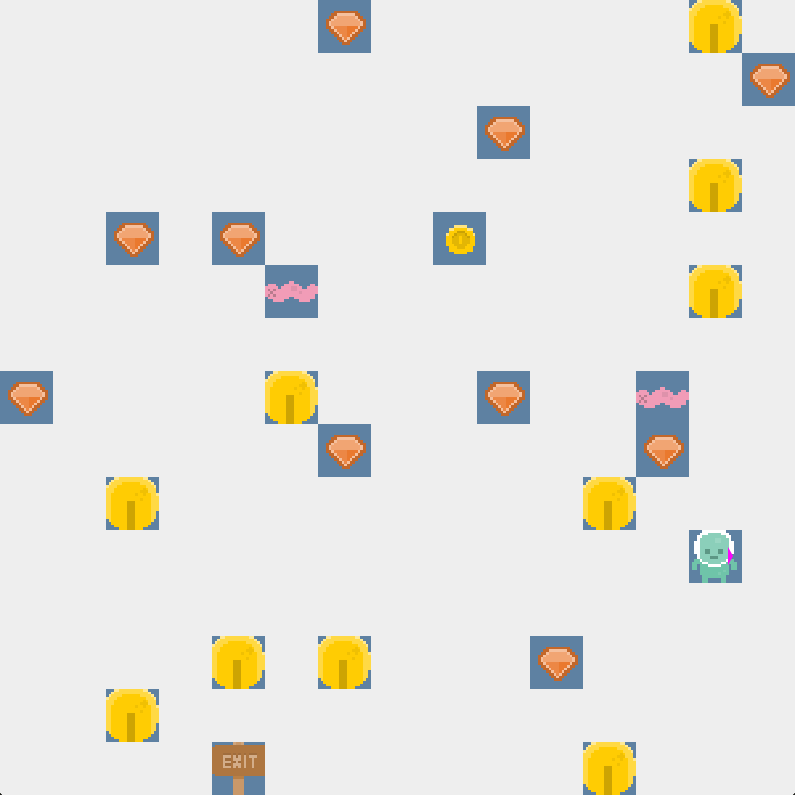
\includegraphics[scale=0.24]{rndgengame.png}
\caption{Visual representation of a randomly generated VGDL game}
\label{fig:gengamescreenshot}
\end{figure}

\subsubsection*{Level generation}
The problem of generating a game is more often than not intimately linked to a generation of levels.
I.e. one could end up with generating game descriptions of high quality games, but if the level descriptions does not fit to the game-play (by being too trivial, or too hard for instance) the games might not be found if searching through a set of generated games.

A simple level generator were constructed with the simple goal of making the randomly generated games playable.
Using each sprites mapping of a game description (defined in the \texttt{LevelMapping}), the generator designates a level using a given size, and inserts a random amount of each sprite, at random positions.

Figure \ref{fig:gengame} shows an example of generated game description-, and Figure \ref{fig:gengamelvl} the level generated for the game, by using process described above.

\begin{figure}[!ht]
\centering
\begin{vgdldesc}[linewidth=14cm]
BasicGame
	SpriteSet
		avatar > HorizontalAvatar img=avatar cooldown=2
		gen1 > Resource limit=10 value=5 img=fire
		gen2 > RandomNPC img=wall
		gen3 > Resource limit=4 singleton=TRUE value=1 img=explosion
		gen4 > OrientedFlicker limit=23 orientation=RIGHT img=water
		gen5 > Spreader limit=14 stype=gen1 img=spaceship
	InteractionSet
		avatar gen1 > killIfFromAbove
		avatar gen2 > killIfOtherHasMore limit=4 resource=gen1
		gen5 gen1 > cloneSprite
		gen4 gen5 > pullWithIt
		gen3 avatar > changeResource value=1 resource=gen1
		avatar gen1 > undoAll
		avatar gen4 > stepBack
		avatar gen5 > stepBack
	LevelMapping
		$ > gen1 
		% > gen2 
		& > gen3 
		' > gen4 
		( > gen5 
	TerminationSet
		SpriteCounter limit=0 stype=avatar win=TRUE 
		MultiSpriteCounter limit=0 stype1=avatar stype2=gen3 win=FALSE 

\end{vgdldesc}
\caption{A randomly generated VGDL game description}
\label{fig:gengame}
\end{figure}

\begin{figure}[!ht]
\centering
\begin{vgdldesc}[linewidth=14cm]
             % 
     %%        
       %'      
             % 
          %    
   %           
            %  
               
  $          & 
               
         % &   
   %           
               
     (  %   A% 
        %   %  
\end{vgdldesc}
\caption{A random generated level description, generated for the VGDL game above}
\label{fig:gengamelvl}
\end{figure}

%\begin{figure}[ht]
%	\centering
%	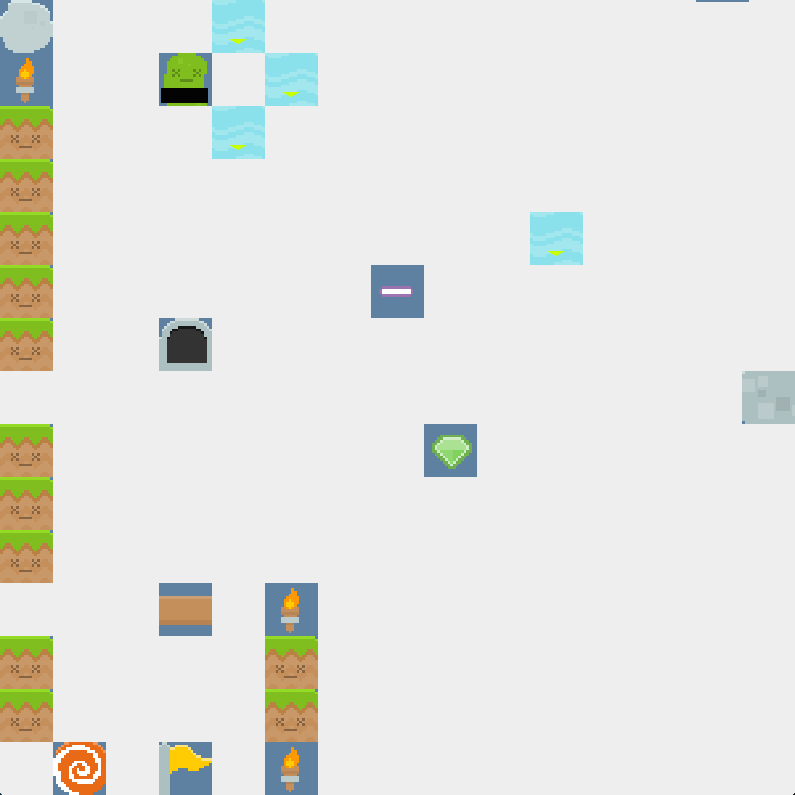
\includegraphics[width=0.45\textwidth]{gengame.png}
%	\caption{Visual representation of one of the 400 randomly generated VGDL games}
%\end{figure}





%------------------------------------------------------------------------------------------------------------------------------%

\section{Playthrough of generated games: Experimental setup}
\label{sec_task1inittestsetup}

Using the generation presented in the previous section, I performed a playthrough test of both the designed- and generated games using different general game playing algorithms (controllers), and discuss different ways to analyse the resulting data.


\subsubsection*{Controllers}
Six different controllers were used to play through the games. 
The controllers use an array of varying approaches, which can be described as a different degree of intelligence. 
One of the more ``intelligent'' controllers used were included in the GVG-AI framework (SampleMCTS), while the remaining were implemented for this work (Explorer, DeepSearch and OneStep).
In addition two extremely simple controllers were created to be used as a basis for ``bad'' play:
1) A \textit{Random} controller, which always returns a random action, and 2) a controller which never acts at all and always return an ``NIL''-action, with the appropriate name \textit{DoNothing}.

%Except for \emph{OneStep-Heuristic}, the controllers only evaluate a given state according to its score and win/loss status.
%Each controller was marked with one of four types of intelligence for later tests: Intelligent (complex searches in game space are taken), semi-intelligent (game space search uses simple approach), random and do-nothing.


\subsubsection*{Generated games}
A set of 130 VGDL games were generated by mutating each of the 13 designed games ten times, using the approach described in the previous section.
400 randomly generated games (generated from scratch), each accompanied with a single randomly generated level of size 15x15, were additionally generated and used in testing.

\subsubsection*{Testing and result analysis}
The six controllers were used to play through the set of human-designed-, mutated and randomly generated games. 
Because of CPU budget limitations each game was played through ten times, with a maximum amount clock ticks of 2000 and 50 ms allowed for each tick.
In addition, a function was implemented to stop playing through games if a clock tick ever takes more than 50 ms, which would happen often when generated games had rules generating too many sprites, which can end up taking a severe amount of time to play through if not discarded quickly.
For each playthrough of games, only the most essential data from the GVG-AI framework was retrieved: The score, the win-lose value, the amount of clock ticks used and a list of actions performed.

A process to analyse the data was built, to calculate averages, standard deviations, max-, minimum and other statistics of each of the values, for each controller, for both each individual game and over a whole set of games.
To more accurately compare the score for the different controllers when playing across a range of different games  I additionally calculate a normalised score using a max-min normalisation ($\frac{score-min}{max-min}$), using the maximum/minimum score for each play through, across the controllers. 
The entropy of actions performed for each playthrough, and averages across playthroughs- or set of games, was additionally calculated

\section{Playthrough of generated games: Results}
\label{sec_task1inittestresults}
Using the setup described above averages of all play-throughs for each controller, is presented and the results compared with each other.

In the results below, a series of data from the generated set of games were removed due to being either too difficult to analyse, or for having certain values which I assess could not possibly result in a quality game.
Namely I remove games by three different considerations: 
1) When a controller was disqualified (because of too many sprites- and/or interactions happening, making a frame using more than the allowed 50 ms), 2) when all controllers get the same score -- and win-rate -- for all playthroughs, and 3) where the game always (for all controllers, for all playthroughs) end in less than 50 clock ticks\footnote{This is also the maximum lifetime of generated \texttt{Flicker}-sprites -- initial trials into VGDL game generation showed that many games was won when a certain type of sprites was all destroyed, but the sprite in question were \texttt{Flicker}s and so even the simplest controller would always win.}.

It should be noted that the uncertainties for average score, clock-ticks and action entropy in the data below assume a normal distribution of the data, which in general is not true, and so these values should be taken with a grain of salt.

\subsubsection*{Designed games}
The six controllers were first of all set to play through each of the human-designed VGDL games.
Below the averages across all the games from the designed set can be seen (Figure \ref{table:designed}). 
Averages across each single game can be seen in Appendix \ref{app_designedresults}, 

The distributions show that there is a large difference between the results of the more intelligent algorithms and that of the intended ´´intended-to-be-bad'' controllers, with both a higher win-rate and a significantly higher average score. 
Surprisingly, the DeepSearch algorithm is has a significant lead over the other algorithms, in spite of its simple approach to selecting actions.

The \textit{clock-ticks} and \textit{action entropy} does not show a similar clear relationship between the more- and less intelligent algorithms, for the collection of all games. 
Examining the results from each game it is noticeable that the profiles for these values (\textit{clock-ticks} and \textit{entropy}) are very different from game to game.


\begin{figure}[!ht]
\centering
\csvreader[tabular=lrrrrr,
    table head=\toprule \textit{\textbf{controller}}
             & \textit{ave. score}
             & \textit{norm. score}
             & \textit{win-rate}
             & \textit{ave ticks}
             & \textit{ave. act entr.},
    late after head=\csvifoddrow{\\\rowcolor{black!5}}{\\\rowcolor{black!25}}\midrule,
    late after line=\csvifoddrow{\\\rowcolor{black!5}}{\\\rowcolor{black!25}},
    late after last line=\\\bottomrule
    ]%
{examplesdata.csv}{1=\Agent,2=\Mean,4=\MeanErr,5=\MMMean,7=\MMMeanErr,8=\WR,9=\WRErr,15=\TicksMean,17=\TicksMeanErr,18=\ActEntMean,19=\ActEntMeanErr}%
{\Agent & \num{\Mean} (\num{\MeanErr}) & \num{\MMMean} (\num{\MMMeanErr}) & \num{\WR} (\num{\WRErr}) & \num{\TicksMean} (\num{\TicksMeanErr}) & \num{\ActEntMean} (\num{\ActEntMeanErr})}%

\caption{Averaged results across all the 13 designed games}
\label{table:designed}
\end{figure}


\subsubsection*{Mutated games} 
After removing games by the requirements mentioned above I was left with a total of 90 game descriptions with some form of playability.
The results of playing through these games with the controllers can be seen in Figure~\ref{table:mutated}. 
The scores have higher means and standard deviations, indicating outliers in the data. 
The ordering of the \emph{normalised score mean} and \textit{win-rate}, however, shows a similar pattern as for the example games, but with the DoNothing controller scoring points and even winning games.
In general the extreme values of norm. score and win-rate is smaller than for the designed set of games.

%all mutations average -- amount of games: 90 -- playthroughs: 10
\begin{figure}[!ht]
\centering
\csvreader[tabular=lrrrrr,
    table head=\toprule \textit{\textbf{controller}}
             & \textit{ave. score}
             & \textit{norm. score}
             & \textit{win-rate}
             & \textit{ave ticks}
             & \textit{ave. act entr.},
    late after head=\csvifoddrow{\\\rowcolor{black!5}}{\\\rowcolor{black!25}}\midrule,
    late after line=\csvifoddrow{\\\rowcolor{black!5}}{\\\rowcolor{black!25}},
    late after last line=\\\bottomrule
    ]%
{mutateddata.csv}{1=\Agent,2=\Mean,4=\MeanErr,5=\MMMean,7=\MMMeanErr,8=\WR,9=\WRErr,15=\TicksMean,17=\TicksMeanErr,18=\ActEntMean,19=\ActEntMeanErr}%
{\Agent & \num{\Mean} (\num{\MeanErr}) & \num{\MMMean} (\num{\MMMeanErr}) & \num{\WR} (\num{\WRErr}) & \num{\TicksMean} (\num{\TicksMeanErr}) & \num{\ActEntMean} (\num{\ActEntMeanErr})}%

\caption{Averaged results across the 90 (out of 130) mutated games, which fulfil the criteria described at the beginning of this section}
\label{table:mutated}
\end{figure}



\subsubsection*{Randomly generated games}
Figure~\ref{table:generated} shows results for the remaining 66 randomly generated games (of 400), with problematic games removed according to the same criteria as above.

The \emph{normalised score means} and \emph{win-rates} both have values that are more closely clustered togther, than in the previous game sets. 
For this set of games the \textit{action entropy} of the intelligent controllers has also fallen quite a bit (relative to the Random-controller), indicating that more of the games have simple solutions to win or increase the score

%2000ticks average -- amount of games: 66 -- playthroughs: 10
\begin{figure}[!ht]
\centering
\csvreader[tabular=lrrrrr,
    table head=\toprule \textit{\textbf{controller}}
             & \textit{ave. score}
             & \textit{norm. score}
             & \textit{win-rate}
             & \textit{ave ticks}
             & \textit{ave. act entr.},
    late after head=\csvifoddrow{\\\rowcolor{black!5}}{\\\rowcolor{black!25}}\midrule,
    late after line=\csvifoddrow{\\\rowcolor{black!5}}{\\\rowcolor{black!25}},
    late after last line=\\\bottomrule
    ]%
{generateddata.csv}{1=\Agent,2=\Mean,4=\MeanErr,5=\MMMean,7=\MMMeanErr,8=\WR,9=\WRErr,15=\TicksMean,17=\TicksMeanErr,18=\ActEntMean,19=\ActEntMeanErr}%
{\Agent & \num{\Mean} (\num{\MeanErr}) & \num{\MMMean} (\num{\MMMeanErr}) & \num{\WR} (\num{\WRErr}) & \num{\TicksMean} (\num{\TicksMeanErr}) & \num{\ActEntMean} (\num{\ActEntMeanErr})}%

\caption{Averaged results across the 66 (out of 400) randomly generated games which fulfil the criteria of a ``not-completely-terrible'' game}
\label{table:generated}
\end{figure}


\subsubsection*{Outcome and graphs}
By examining the graphs below (especially Figure \ref{graph:maxminmean} and Figure \ref{graph:winrate}) presenting the data discussed, it is clear that there is some relationship between the performance profiles of playing with controllers of different types, on different set of games.
However it should be noted here that some games from both the mutated- and generated game-set, contains games, which when examined by themselves have similar distributions as the average designed game (these will be discussed below).

\begin{figure}[!ht]
\centering
\begin{tikzpicture}[font=\small, scale=1]
  \begin{axis}[
	ybar, bar width=0.38cm,
	xtick=data, xtick pos=left,
	ylabel=Average normalised score, ymajorgrids, ymin=0, ymax=1,
	symbolic x coords={Explorer,DeepSearch,MCTS,Onestep, Random, Do Nothing},
	width=\textwidth, height=6cm,
	legend style={
	  overlay, area legend, anchor=north,legend columns=1, at={(0.913,1.00)} %, at={(0.5,-0.15)}
	},
	legend image code/.code={%
          \draw[#1, draw=none] (0cm,-0.1cm) rectangle (0.6cm,0.1cm);
        }
]
    \addplot[fill=LightBlue, error bars/.cd, y dir=both, y explicit] table [x=Agent:, y=MaxMinN-Mean:, y error=MaxMinN-SE:, col sep=comma] {examplesdata.csv};
    \addplot[fill=LighterBlue, error bars/.cd, y dir=both, y explicit] table [x=Agent:, y=MaxMinN-Mean:, y error=MaxMinN-SE:, col sep=comma] {mutateddata.csv};
    \addplot[fill=LightestBlue, error bars/.cd, y dir=both, y explicit] table [x=Agent:, y=MaxMinN-Mean:, y error=MaxMinN-SE:, col sep=comma] {generateddata.csv};
\legend{designed,mutated,generated}
\end{axis}
\end{tikzpicture}
\caption{Averaged normalised score across all games of the three different set of games: Designed-, mutated- and completely generated games}
\label{graph:maxminmean}
\end{figure}


\begin{figure}[!ht]
\centering
\begin{tikzpicture}[font=\small, scale=1]
  \begin{axis}[
	ybar, bar width=0.38cm,
	xtick=data, xtick pos=left,
	ylabel=Average normalised score, ymajorgrids, ymin=0, ymax=1,
	symbolic x coords={Explorer,DeepSearch,MCTS,Onestep, Random, Do Nothing},
	width=\textwidth, height=6cm,
	legend style={
	  overlay, area legend, anchor=north,legend columns=1, at={(0.913,1.00)} %, at={(0.5,-0.15)}
	},
	legend image code/.code={%
          \draw[#1, draw=none] (0cm,-0.1cm) rectangle (0.6cm,0.1cm);
        }
]
    \addplot[fill=LightBlue, error bars/.cd, y dir=both, y explicit] table [x=Agent:, y=Winrate:, y error=Winrate-SE:, col sep=comma] {examplesdata.csv};
    \addplot[fill=LighterBlue, error bars/.cd, y dir=both, y explicit] table [x=Agent:, y=Winrate:, y error=Winrate-SE:, col sep=comma] {mutateddata.csv};
    \addplot[fill=LightestBlue, error bars/.cd, y dir=both, y explicit] table [x=Agent:, y=Winrate:, y error=Winrate-SE:, col sep=comma] {generateddata.csv};
\legend{designed,mutated,generated}
\end{axis}
\end{tikzpicture}
\caption{Averaged win-rate for the three sets}
\label{graph:winrate}
\end{figure}



\begin{figure}[!ht]
\centering
\begin{tikzpicture}[font=\small, scale=1]
  \begin{axis}[
	ybar, bar width=0.38cm,
	xtick=data, xtick pos=left,
	ylabel=Average normalised score, ymajorgrids, ymin=0, ymax=3000,
	symbolic x coords={Explorer,DeepSearch,MCTS,Onestep, Random, Do Nothing},
	width=\textwidth, height=6cm,
	legend style={
	  overlay, area legend, anchor=north,legend columns=1, at={(0.913,1.00)} %, at={(0.5,-0.15)}
	},
	legend image code/.code={%
          \draw[#1, draw=none] (0cm,-0.1cm) rectangle (0.6cm,0.1cm);
        }
]
    \addplot[fill=LightBlue, error bars/.cd, y dir=both, y explicit] table [x=Agent:, y=Mean tick:, y error=Std tick err:, col sep=comma] {examplesdata.csv};
    \addplot[fill=LighterBlue, error bars/.cd, y dir=both, y explicit] table [x=Agent:, y=Mean tick:, y error=Std tick err:, col sep=comma] {mutateddata.csv};
    \addplot[fill=LightestBlue, error bars/.cd, y dir=both, y explicit] table [x=Agent:, y=Mean tick:, y error=Std tick err:, col sep=comma] {generateddata.csv};
\legend{designed,mutated,generated}
\end{axis}
\end{tikzpicture}
\caption{Averaged clock tick for the three sets}
\label{graph:clocktick}
\end{figure}



\begin{figure}[!ht]
\centering
\begin{tikzpicture}[font=\small, scale=1]
  \begin{axis}[
	ybar, bar width=0.38cm,
	xtick=data, xtick pos=left,
	ylabel=Average normalised score, ymajorgrids, ymin=0, ymax=1,
	symbolic x coords={Explorer,DeepSearch,MCTS,Onestep, Random, Do Nothing},
	width=\textwidth, height=6cm,
	legend style={
	  overlay, area legend, anchor=north,legend columns=1, at={(0.913,1.00)} %, at={(0.5,-0.15)}
	},
	legend image code/.code={%
          \draw[#1, draw=none] (0cm,-0.1cm) rectangle (0.6cm,0.1cm);
        }
]
    \addplot[fill=LightBlue, error bars/.cd, y dir=both, y explicit] table [x=Agent:, y=Actions entropy:, y error=Actions entropy err:, col sep=comma] {examplesdata.csv};
    \addplot[fill=LighterBlue, error bars/.cd, y dir=both, y explicit] table [x=Agent:, y=Actions entropy:, y error=Actions entropy err:, col sep=comma] {mutateddata.csv};
    \addplot[fill=LightestBlue, error bars/.cd, y dir=both, y explicit] table [x=Agent:, y=Actions entropy:, y error=Actions entropy err:, col sep=comma] {generateddata.csv};
\legend{examples,mutated,generated}
\end{axis}
\end{tikzpicture}
\caption{Averaged action entropy for the three sets}
\label{graph:acten}
\end{figure}


\section{Discussion of initial test results}
\label{sec_task1discussion}
The results display some interesting patterns. 
Especially the win-rates suggest a relationship between intelligent controllers' success and better game design; for better designed games, the relative performance of different types of algorithms differ more. 
This supports the hypothesis that relative algorithm performance profiles can be used to differentiate between games of different quality. 
In randomly generated games, which arguably tend to be less interesting than the others, smarter controllers (e.g. Explorer and MCTS) do only slightly better than the worse ones (i.e. Random and DoNothing). 
This is due to a general a lack of consistency between rules generated in this manner. 
Mutated games, however, derive from a designed game. 
Therefore, they maintain some characteristics of the original idea, which can improve the VGDL description's gameplay and playability. %!!!!!!!!!!!!!!!KOPIERET FRA ARTIEKL!!!!!!!!!!!

While it is possible that random actions can result in good outcomes, this chance is very low, especially when compared to the chance of making informed decisions. 
In spite of that both Random and DoNothing do fairly well in randomly generated games. 
The performance of DoNothing emerges as a secondary indicator of (good) design: 
In human-designed games, DoNothing very rarely wins or even scores.

\subsubsection*{Human play of generated games}
As mentioned in Section \ref{sec_task1inittestresults} there was a series of generated games with performance profile basically indistinguishable from the designed games.
I decided on examining many of these games further by studying their game descriptions, and playing the games with visuals enabled, both with AI controllers and human players. 
%(SCREEEEEENSHTOS PL0X!!!)
Besides a few mutated games which kept most of the original rules, and therefore were successful games, the tested generated games were in general too trivial and aimless to be entertaining.
However, by also comparing these games with other without the ``well-formed'' performance profiles, it became clear that performance profiles of algorithms could at least be used to separate ``not-completely-bad'' games from terrible games. 

This however gives an indication of in important assumption: That I can assume that the generated games, at least from the randomly generated set, are of a overall low quality.
I will carefully use this assumption to construct an evaluation function for games, in the next chapter,

Besides the above, a few re-occurring problems was found in the generated games.

\begin{itemize}
\item Sprites often completely leave the level playing field. 
For instance because they are of the \texttt{Missile}- or \texttt{Fleeing} (which tries to move away from a specified sprite each frame) sprite classes.
\item The game can only be won in the first few (<50) frames. 
Because sprites disappear before that (for instance  because the sprite is \
\item There is too much purposeless and arbitrary going on: 
Often some sprites can not be interacted with at all, and just wander around on the screen, or they can only be interacted by certain non-avatar sprites.
\item Several of the sprites- and/or rules are never used.
\end{itemize}




%------------------------------------------------------------------------------------------------------------------------------%
%------------------------------------------------------------------------------------------------------------------------------%
%------------------------------------------------------------------------------------------------------------------------------%

\chapter{Evaluation and evolution of games}
\label{ch_task2}

The initial tests of the previous chapter shows that there is reason to explore the relationship of AI's perfomance profiles to analyze a given VGDL game, and give some indications of interesting statistical values to analyse.

This chapter focuses on, using the results of the previous chapter, creating a fitness function to analyse different generated games, allowing a evolutionary algorithm to evolve well-designed games, by creating and evolving VGDL game descriptions.
The resulting generated games are then discussed in detail.

\section{Fitness function: Introduction}
\label{sec_task2intro}
The tests of the previous chapter indicates that the relationship between general game playing controllers performance could potentially be used to determine the quality of games. 
To make it possible to use the performance relationships, while not overfitting the parameters to the small set of ``good'' data points (13 human-designed games), it is necessary to find the most important and selective statistical values from playthrough results for use in a fitness function, while trying to exclude statistics that do not signify game quality.

As mentioned in Section \ref{sec_task1discussion} the score and win-rate seems to have the most distinct distributions for the different type of games, with human-designed games all having a significant difference between e.g. the Explorer- and Random controller, making them interesting to use for an evaluation function.
The \textit{action entropy} might also be appropriate to use, but the difference in the statistical distributions are much smaller for these values.

Limiting fitness features to score and win-rate, there is still an enormous amount of possible ways to calculate features-values for the fitness function.
For instance, I could have a feature for the difference in average score between every single controller but it would result in $\binom{6}{2}=15$ features for a single statistic.
Also, I could use a series of different values simply to compare the score: \textit{minimum}- and \textit{maximum} score, \textit{standard deviation} of score, \textit{median}, \textit{quartiles} or any form of normalised score, and of course I could  use combined values for the features, e.g. the score increase per clock tick.

Additionally it is not straightforward to calculate a feature even after deciding the controllers and value to compare (e.g. score or clock ticks between Explorer and Random).
I could use a simple relative difference formula (e.g. $f=\lvert\frac{a-b}{max(a,b)}\rvert$), and use the result as a feature, but it might make more sense to hand-craft each feature to a specific goal, for instance for the action entropy it seems (from the data of the last chapter) designed games cause the intelligent controllers to have a similar value as the Random controller, while the same is not true for the randomly generated games -- in the generated games the intelligent controllers often find a simple solution requiring similar actions.
A feature could therefore be made to have a value of 1 if the entropies are the close (and going toward 0/-1 when random has a higher entropy), while not rewarding the game for having the intelligent controllers action entropy be higher than Random (which the data do not show as a relationship in designed games).

Also, how each fitness feature adds to the complete fitness function is not straightforward.
One could use a simple sum of each chosen feature, maybe with a weight constant attached signifying how much each feature adds the overall value ($f = w_1a_1+...+w_na_n$), but the approach can have the outcome of some features overruling others.

In the following I will try to shed light on which features are the most interesting, by both analysing the data in more detail, and by evolving games using the features.



\section{Performance relationship analysis}
\label{sec_task2fitnessSelection}
%This section describes the process in which the initial fitness features were selected (i.e. before starting to evolve games using the fitness function).
Since the relationships between controllers acting intelligent, and acting random or doing nothing, seems to be a possible indication of game quality, an analysis of the relationship between different controllers using varying values was performed.
As indicated in the previous section, choosing how to evaluate game for the fitness function almost certainly have an element of  subjectivity. 
To make an as informed decision as possible I ran a series of test described below, using different features, evolving weights for the features, and examine the results.

In the following I repeatedly to use a \textit{relative difference}-function ($f=\lvert\frac{a-b}{max(a,b)}\rvert$) to compare statistical values  between controllers performance results, retrieved from playthroughs.
Additionally I chose to simply construct the fitness function as a sum of the individual features.

Also, the assumption that the games from the generated- and mutated set simply are of a low quality (discussed in Section \ref{sec_task1discussion}), is used throughout the following analysis.

\subsubsection*{Analysis of possible relationship features}
As mentioned in the previous sections, the relationship of score and win-rate between controllers seems to be obvious choices to adopt as fitness features.
Also, the there seems to be a consistent difference in the values between the intelligent controllers (especially Explorer and DeepSearch) and the less intelligent ones: The OneStep, Random and Do Nothing-controllers.

To measure the strength of different possible choices I performed a small test, counting how often a specific intelligent controller has a higher value than a simple one, and calculating the average relative difference between the pair. 
The results can be seen in Figure \ref{table:simplefeatureanalysis}.


\begin{figure}[!ht]
\centering
\csvreader[tabular=l|rr|rr|rr|,
    table head=\toprule \textit{\textbf{data type}} & \multicolumn{2}{c|}{Designed} &\multicolumn{2}{c|}{Mutated} & \multicolumn{2}{c|}{Rnd. gen.} \\
             & \textit{count} & \textit{diff.} & \textit{count} & \textit{diff.} & \textit{count} & \textit{diff.},
    late after head=\csvifoddrow{\\\rowcolor{black!5}}{\\\rowcolor{black!25}}\midrule,
    late after line=\csvifoddrow{\\\rowcolor{black!5}}{\\\rowcolor{black!25}},
    late after last line=\\\bottomrule
    ]%
{testcounts.csv}{1=\DataType, 2=\CountA, 3=\FracA, 4=\CountB, 5=\FracB, 6=\CountC, 7=\FracC}%
{\DataType & \CountA & \FracA & \CountB & \FracB & \CountC & \FracC}%

\caption{Simple analysis of possible fitness values}
\label{table:simplefeatureanalysis}
\end{figure}

Some of the features in the table immediately seems interesting and significant, for instance the score average- and win-rate difference between the intelligent- and the DoNothing controller is consistently higher for the intelligent controllers, while the same is not true for several of the games from the mutated- and randomly generated set.
The average clock ticks between, for instance Explorer and OneStep additionally could be interesting to use as an indication of a bad game, since the value is never higher for OneStep in the generated game set.
However the actual relative difference between the controllers is tiny, and so the relationship might not be that significant. 
Also the designed games do not have a clear relationship profile for the clock ticks (as discusses in Section \ref{sec_task1discussion}).

%The features above (and other sets) were analysed by data mining techniques -- i.e classification processes were to used to see if it was possible to differentiate between the designed- and generated set of games.


\subsubsection*{Analysis of feature sets}
From the analysis of features, a selection of interesting values are available, and of these I continuously tested the results of  selecting different sets of features (between 2-20) of relative difference values between pairs of controllers.

From the varying sets of feature selections, I first of all calculated and compared the resulting fitness (by summing the features) of games from both the designed- and generated set, noticing how each game was scored -- while examining the data from high-fitness generated-, and low-fitness designed games further.

I continuously tried evolving a set of weights for individual features, to balance the contribution from each type of values using a CMA-ES algorithm\footnote{https://www.lri.fr/~hansen/cmaes\_inmatlab.html}.
For this task another problem arise however: Creating a fitness function to score a chosen set of weights.
Several different approaches were tried for this task, but all relying on the assumption that all the games from the randomly generated set of Chapter \ref{ch_task2} were of a low quality.
Using the assumption, the fitness was increased if the set of weights caused the overall fitness of the designed games to be larger than for the randomly generated set (from Chapter \ref{ch_task1}).

Because the amount of games assumed to be of a good quality were rather small (13 human-designed games) this approach was discarded, in fear of overfitting the fitness function to the data points.


\subsubsection*{Outcome}
From the above analyses I decided to only use two different relative difference values from performance profiles of the controllers, to use in the fitness function, both having a unique form in the designed set of games, while not appearing similarly in the generated set of games.

The chosen features were:
\begin{description}
\item[A function comparing score means] between DeepSearch and DoNothing. Returning the relative difference between the two values.
\item[A features comparing win-rates] between DeepSearch and DoNothing. Returning the relative difference between the two values.
\end{description}

Where the total fitness of a game was given by the sum of the two values.
Using these features, 12 of the designed games has a ``perfect score'' of 1, while the game DigDug only score 0.5 (since the DeepSearch controller was never able to win).
30 of the mutated games has a score of 0.95 or higher (23 has perfect score), while only 4 of the generated games has a fitness above 0.5 (however these are all perfect scores of 1).

I tested many of the games from the mutated set of games, but they can in general be described as a twist on the original games, but with some game-breaking element (for instance the avatar suddenly becomes able to walk through wall, dirt or water), and because of the sheer amount of games with high fitness they become difficult to analyse thoroughly (too see if any of them actually contains interesting game design).

The four randomly generated games additionally were not much fun to test, and in general they contained similar problems as those discussed at the end of the last chapter (Section \ref{sec_task1discussion}): They were too trivial, and the winning solutions caused the game to end too quickly.
Of the games, \texttt{gen_game44} probably contains the most interesting game design (see Figure \ref{fig:gengame44}).
The player avatar can only move left and right, but also place ground sprites. 
There is a ``door'' sprite falling down slowly from above, and the goal is simply to place a ground sprite below the door.
The crate- and gem sprites has no effect in the game.

\begin{figure}[!ht]
\centering
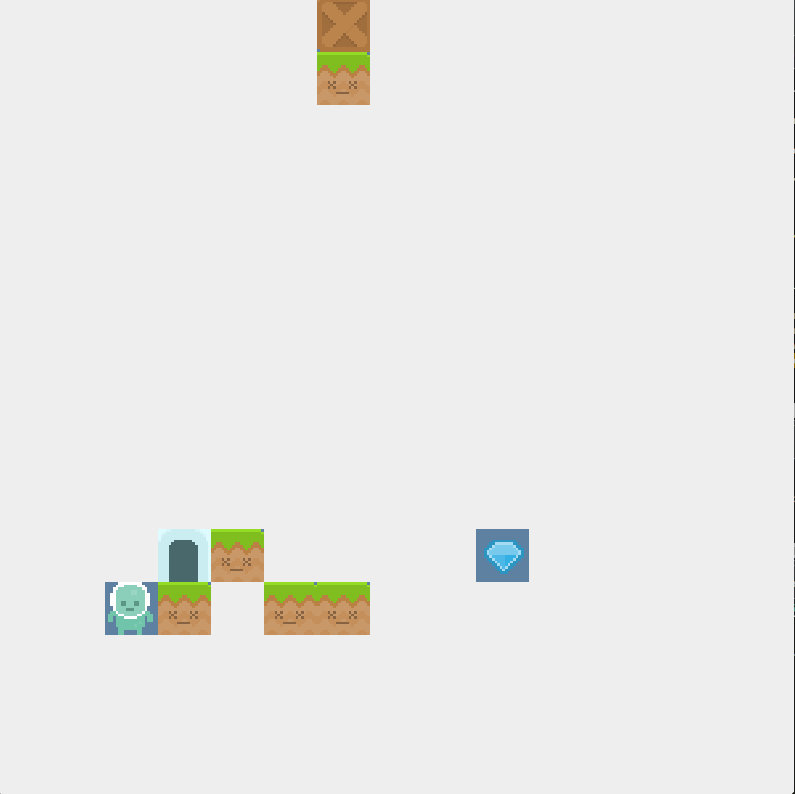
\includegraphics[scale=0.24]{gengame44.png}
\caption{Screenshot of a generated VGDL game (\texttt{gen_game44}), where the DeepSearch algorithm plays consistently better than DoNothing}
\label{fig:gengame44}
\end{figure}



%------------------------------------------------------------------------------------------------------------------------------%


\section{Further selection of features}
\label{sec_task2furtherfeatures}

After examining the resulting fitness values from generated VGDL games, and increasingly starting to evolve games using the fitness function (described in the next section), it became clear that I would need to introduce more fitness features, especially using non-relative values -- i.e. instead of comparing controllers' results, using for instance averaged results across the controllers or only use results from a single controller.

The first insight was (also discussed in Chapter \ref{ch_task1}) that games where the intelligent controllers can win too quick -- I decided on 50 clock ticks -- should have a reduced fitness.
A correlated problem is that the intelligent controllers often has a low \textit{action entropy} in these games, but this is seemingly directly related to the fact that they can win with only a few precise actions.

The second insight was that the the intelligent controllers is often able to both win AND lose in many of the designed games (controllers standard deviation of win-rate above zero), while this happens rarely in the generated games. 
Although this is not true for all of the designed games, it is able to give an indication of the difficulty of a game which seems to otherwise be missing.

As a result, the fitness function used to evolve games had the following form: \\

$fitness = \frac{relDiff(\text{average score}) + relDiff(\text{average wins}) + \text{[can win in 50 ticks]} + \text{[can win and lose]}}{4}$ \\

Where [can win in 50 ticks] returns -1 if a  controller is able to win in less than 50 clock ticks, and otherwise gives 1, and [can win and lose] similarly returns either a 1 or -1 if the standard deviation of win-rate is above 0 (1 if true).
The resulting fitness is a numerical value between -1 and 1.

In addition a game is automatically given a fitness of -1, if it does not fulfil the criteria used in accepting games in Chapter \ref{ch_task1}: 
That the controllers are not disqualified, that the score and wins is not always the same, and that the controllers do not all finish in less than 50 clock ticks.

%------------------------------------------------------------------------------------------------------------------------------%

\section{Evolution of games: Setup}
\label{sec_task2evolvingGames}
A process for generating and evolving new VGDL games were built using the fitness function found in the previous section.
Two different approaches were again used to create new game description:
1) Evolving from an existing, human-designed game description, using human-designed levels, and 2) evolving from randomly generated games, using randomly generated levels.

In both approaches a simple evolution strategy (ES) approach, using mutation- and crossover operations across several generations, in order to increase the fitness of a population (of games).
For each generation a population of game descriptions are tested using the two controllers DeepSearch and DoNothing, and a fitness is calculated for each game, with the lowest fitness games being removed from the population.
As in the previous chapter, only the interaction rules (of the \texttt{InteractionSet}) were evolved over each generation.

Because of CPU scheduling issues\footnote{The problem is mostly that it just takes a lot of time for intelligent controllers to play through each game. Each controller is allowed up to 50 ms per tick, and so even with a maximum of 800 ticks, playing through a game 6 times can take up to $50ms \cdot 800 \cdot  6 = 240s$. With a population size of 50 over 15 generation, a single game can in the worst case take up to 50 hours to evolve.} the populations size was limited to 50, with 25 members always surviving each generation, with a limit of 15 generations.
Additionally the maximum amount of clock ticks for playthroughs was limited to 800.

The evolution process was stopped when the highest fitness stopped increasing over 10 generation, when the best games fitness were above 0.98 (an almost perfect score), or when the 20 generations allowed were over.

%\subsubsection*{Evolving designed games}


\subsubsection*{Evolving randomly generated games}
An additional process was used to evolve games from a randomly generated game (using the generation process of Section \ref{sec_task1genApproach}), which also requires a level generated for the description, to allow playing it.
Since the evolution process itself is only focused on changing the interaction rules, it should be certain that the \texttt{SpriteSet}, \texttt{TerminationSet} and the level description (and \texttt{LevelMapping} are well-formed, so the evolution strategy is actually able to find games of high fitness.

Therefore a process was built to first continuously generate a new game- and level descriptions, playing through them with the controllers, and then checking for 1) that the fitness is above -1 (which simply means that the minimum criteria for a game has been fulfilled), and 2) that intelligent controller was actually able to win.
From the results of Section \ref{sec_task1inittestresults} I know that DeepSearch has a average win chance of 11\% in the set of randomly generated games, however, where 334 games has already been removed for not fulfilling the minimum criteria, and so we can expect that at least $\frac{66}{400}\cdot 11\% = 1.8\%$, or every 55th game description, will be fulfil the criteria and be selected to evolve from.

As mentioned in the discussion of the results of Chapter \ref{ch_task1} the previous randomly generated games had a problem of sprites leaving the playing field.
To counter this an interaction rule was made for each sprite in the generated descriptions, making sprites take a step back if trying to move out of the level.

%\subsubsection*{Evolution process}
%
%The figure below shows the process which was used in both evolution approaches.
%
%HERE SHOULD BE A PICTURE OF THE EVOLUTION PROCESS
%
%Generate game --> if not player runs out of time --> if not any sprites out of bounds --> get results --> if no disq --> if no low time wins --> if no all squares equal


%------------------------------------------------------------------------------------------------------------------------------%
\section{Evolution of games: Results}
\label{sec_task2evolvingGames}
Because of the ability of the evolution strategy to return early if the fitness increased over 0.98, a large amount of game description were generated, especially when generating game by mutating the game Boulderdash, were a ``perfect'' fitness games (fitness of 1) were often found in the first generation -- which however caused them to only have a small number of differences from the original game description of Balderdash.
A series of 54 games were generated and evolved over 4 days, 45 by evolving from the human-designed game Boulderdash, and 9 by evolving games from a randomly generated game- and level description.
Of these games 40 mutated-, and 6 randomly generated games had a perfect, or near-perfect fitness of >0.98, making them the most interesting to examine further.

Playing through an array of the Boulderdash mutations I noticed that the games still had many of the problems first discussed in Chapter \ref{ch_task1} when examining mutated games:
The mutation often cause certain important game rules of the originals to be broken -- suddenly the player can walk through walls- or boulders, gems does not disappear after they have increased the players score, or enemies can no longer harm the player.
With that being said, some of the games certainly contain some interesting aspects.
In \texttt{boulderdash_mut09} (see Figure \ref{fig:evolved_boulderdash} for changes in the games' rules), which is also one of the better games\footnote{Gems do no disappear when collected, making the player able to win very quickly (one just has to stand still on gem for a second, and then head for the exit), but at the same time enemies can walk through ground making the game has some sense of challenge and difficulty -- compared to the other generated games.}, the avatar has gained an ability to push boulders making them glide across the level with the ability to kill certain enemies.
However, the enemies that can be killed by the boulders no longer harm the avatar, and so the new ability does not cause much change to the actual game.

\begin{figure}[!ht]
\centering
\begin{vgdldesc}[linewidth=14cm]
InteractionSet
	dirt avatar > killSprite									
	dirt sword  > killSprite
	diamond avatar > collectResource
	diamond avatar > killSprite scoreChange=2
	moving wall > stepBack
	moving boulder > stepBack
	avatar boulder > killIfFromAbove scoreChange=-1
	avatar butterfly > killSprite scoreChange=-1
	avatar crab > killSprite scoreChange=-1
	boulder dirt > stepBack
	boulder wall > stepBack
	boulder diamond > stepBack
	boulder boulder > stepBack
	enemy dirt > stepBack
	enemy diamond > stepBack
	crab butterfly > killSprite
	butterfly crab > transformTo stype=diamond scoreChange=1
	exitdoor avatar > killIfOtherHasMore resource=diamond limit=9
	
	-->
	
InteractionSet	
	dirt avatar > killSprite
	dirt sword > killSprite
	boulder avatar > attractGaze
	dirt diamond > killIfFromAbove
	moving wall > stepBack
	moving boulder > stepBack
	avatar boulder > killIfFromAbove scoreChange=-1
	butterfly dirt > killIfHasMore limit=15 resource=diamond
	avatar crab > killSprite scoreChange=-1
	boulder dirt > stepBack
	butterfly avatar > killIfFromAbove
	sword crab > cloneSprite
	boulder boulder > stepBack
	avatar EOS > killIfHasLess limit=13 resource=diamond
	diamond dirt > transformTo stype=diamond
	crab butterfly > killSprite
	diamond avatar > collectResource
	exitdoor avatar > killIfOtherHasMore limit=9 resource=diamond
	butterfly boulder > killSprite
\end{vgdldesc}
\caption{The original- and evolved set of interaction-rules of a VGDL description, generated by mutating the description of Boulderdash.}
\label{fig:evolved_boulderdash}
\end{figure}

I played through all of the 6 games of ``perfect'' fitness evolved from randomly generated descriptions, which in general has a more unique design that the Boulderdash-evolved descriptions.
The outcome of several of the games are partly- or completely random, no matter what the player does the results are the same: 
This is likely a product of using a rather small statistical sample when playing through each game (6 playthroughs for each controller).
The games are overall quite simple, but several of them contain some interesting game design for human players -- some which seemingly has appeared by accident:

In the evolved game  \texttt{evol_game01} (see Figure \ref{fig:evolved_random_game_desc} (description) and Figure \ref{fig:evolved_random_game_screenshot} (screenshot)) the goal is to kill a block of dirt that whizzes around the level, trying to flee from the avatar.
However, true to the action-arcade genre of the game, the player can additionally increase his/her score by moving the avatar to a laser-sprite (\texttt{gen2} in the description). 
Only one laser-sprite can exist in the level -- because of its parameter \texttt{singleton=TRUE}, and the player can only increase his/her score by repeatedly going to each laser that is spawned.
%Only one laser-sprite can exist in the level (because of is parameter \texttt{singleton=TRUE}), and the player can only increase his score by repeatedly going to each laser-sprite that is spawned.
%However the game has an interesting feature: If the player picks up a laser in the same position of a previously picked up laser, the player loses all his points.
The game \texttt{evol_game02} is rather simple, in that the goal is simply to kill the avatar, which can be achieved by walking to the ``cog'' sprite (at the top of the screen in Figure \ref{fig:evolved_random_game_screenshot2}.
However the game is lost if the bat sprite (a \texttt{RandomNPC}) ever collides with the same object, making the outcome rather random.





\begin{figure}[!ht]
\centering
\begin{vgdldesc}[linewidth=14cm]
BasicGame
	SpriteSet
		avatar > MovingAvatar img=avatar
		gen1 > Passive img=honey
		gen2 > Resource limit=4 singleton=TRUE img=missile value=2
		gen3 > Immovable img=pellet
		gen4 > Bomber orientation=DOWN stype=gen5 img=frog prob=0.22090000000000004
		gen5 > Spreader limit=33 stype=gen2 img=fire
		gen6 > Fleeing stype=avatar img=dirt
	InteractionSet
		gen6 gen4 > attractGaze
		avatar EOS > killSprite
		gen5 EOS > wrapAround
		gen1 gen3 > killIfHasLess limit=3 resource=gen2
		gen2 avatar > transformTo stype=gen1 scoreChange=2
		gen2 avatar > wallStop
		gen2 avatar > changeResource resource=gen2 value=0 scoreChange=7
		gen6 gen2 > killIfOtherHasMore limit=0 resource=gen2
		avatar EOS > stepBack
		gen1 EOS > stepBack
		gen3 gen3 > stepBack
		gen3 EOS > stepBack
		gen1 gen1 > spawnIfHasMore limit=11 stype=gen6 resource=gen2 scoreChange=-2
		gen5 EOS > stepBack
		gen6 EOS > stepBack
		gen2 gen5 > collectResource
	LevelMapping
		$ > gen1 
		% > gen2 
		& > gen3 
		' > gen4 
		( > gen5 
		) > gen6 
	TerminationSet
		SpriteCounter limit=0 stype=gen6 win=TRUE 
		SpriteCounter limit=0 stype=avatar win=FALSE 
\end{vgdldesc}
\caption{The VGDL game description for the evolved game \texttt{evol_game01}}
\label{fig:evolved_random_game_desc}
\end{figure}

\begin{figure}[!ht]
\centering
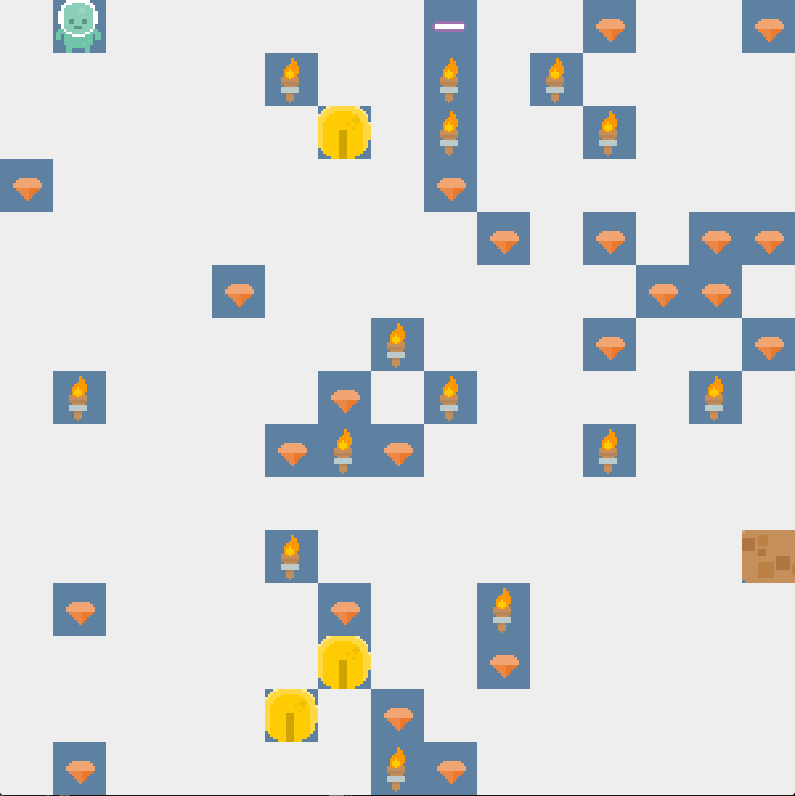
\includegraphics[scale=0.24]{coolgame1.png}
\caption{Screenshot of a evolved-from-random-generated VGDL game (\texttt{evol_game01}) with a fitness score of 1}
\label{fig:evolved_random_game_screenshot}
\end{figure}


\begin{figure}[!ht]
\centering
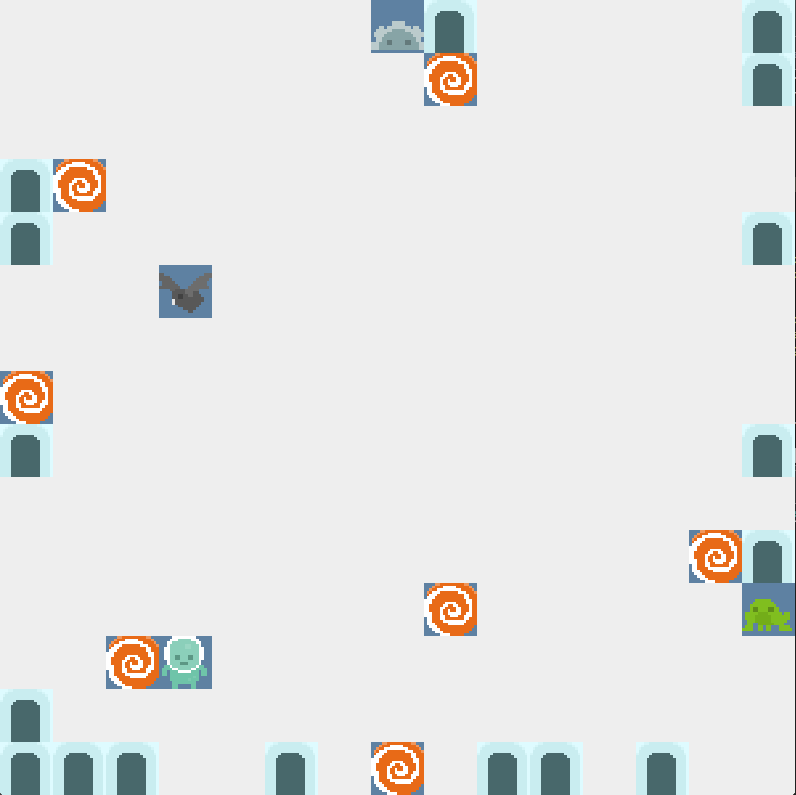
\includegraphics[scale=0.24]{coolgame2.png}
\caption{Screenshot of a evolved-from-random-generated VGDL game (\texttt{evol_game02}) with a fitness score of $\approx$0.98}
\label{fig:evolved_random_game_screenshot2}
\end{figure}


%HERE GOES A GRAPH OF HOW FITNESS INCREASES OVER TIME IN EVOLUTION


%------------------------------------------------------------------------------------------------------------------------------%

\section{Discussion of results}
\label{sec_task2discussion}
Many of the games generated by in this chapter definitely have some interesting properties and features, but overall the VGDL game generation process was not able to create any complete games of a high enough quality to compare with other games of the genre.
Additionally the generator was only able to find games with interesting qualities, and did not guarantee that each generated games were any good. 
The generator was simply able to find sets of games in the space of VGDL game descriptions with a significantly higher chance of quality, than for completely randomly generated games. 

To be able to increase the quality of the game generator one would almost definitely need to refine- and extend the fitness function, which could identify many more aspects of games- and playthroughs of games.
For instance, one could examine how each controller increased its score across a playthrough, th proportion of sprites- and rules that have been in use in the game, the amount of sprites that has left the level field, or the amount of objects that have been killed or created.
I have implemented functions for retrieving several more value (like these) in the GVG-AI framework, but initial examination of the values did not show any clear form or profile, for the human-designed set of games\footnote{https://docs.google.com/spreadsheets/d/1HAuIdXBcv4MXTlerkSqz8tK-zXMypzzQAU8sRlt95TA/edit?usp=sharing}.



%------------------------------------------------------------------------------------------------------------------------------%
%------------------------------------------------------------------------------------------------------------------------------%
%------------------------------------------------------------------------------------------------------------------------------%

\chapter{Puzzle generation}
\label{ch_task3}
In this chapter I will explore the prospect of automatically generating VGDL puzzle games- and levels.
First an array of human-designed puzzle games will be examined using a general puzzle solving algorithm.
Then, using the results of the algorithm, a general level generator for puzzle games will be introduced, and generated levels for designed games presented.
At the end, a process for both generating a (puzzle) game description and evolving a level, will be shown and the results of the generator discussed.

\section{Puzzle analysis introduction}
\label{sec_task3intro}
To analyse and generate puzzle games more quickly, my implementation of VGDL: SimpleVGDL (Section \ref{sec_fastvgdl}), was used to test- and generate levels, instead of the GVG-AI framework.


%\subsubsection*{Definition of games}
%The games described in this section are games where the puzzles are the only game-play. There is no fast movement, or quick reaction time required to win. Additionally, because the games are described using the GVG-AI framework, the games focus around a player avatar which can only move up, down, left or right (also, in the games described below, all movement are from one game-tile to another).

\subsubsection*{Games} 
From the GVG-AI framework (Section \ref{sec_gvgaiframework}) and my own additions (Section \ref{sec_writingnewvgdl}), there is a total of 10 puzzle games to use in the following analysis.

However, several of the games were deemed unfit for a complete examination.
Some, because the levels were too difficult for the a breadth first search algorithm to have a chance (Bolo Adventures and Chip's Challenge).
Three other games were removed from a more technical reason: 
The games Bombuzal, ZenPuzzle and Painter all has a continuous creation of \texttt{Flicker}-sprites, which (as mentioned in Section \ref{sec_creatingnewcontrollers})  halts the PuzzleSolver in its progress.
Because of this, only the following five games were used as a base-line for ``good'' puzzle games: Bait, Brainman, The Citadel, Sokoban and Modality.


%\subsubsection*{Solving puzzle games} 
%As mentioned in (WHERE ITS MENTIONED), the controllers from the GVG-AI competition are not well-suited for playing puzzle games, because the goal can often only be achieved by applying a specific series of moves, which the controllers are not very good at.
%Two general puzzle solving algorithms were implemented. The overall goal of the controllers were to analyze the game as much as possible, rather than finding a solution fast, or using as low memory as possible
%They controllers use fact that wall-sprites in the different games always push back the player, and so the controllers do not try to move into a wall -- this is achieved by storing the positions of every wall-sprite at the start of the game. 
%Also, the controllers store each path it is had tried. For each path a game state is calculated and stored, by finding the position and type of each (non-wall) sprite in the game. A path is cut off if the calculated game state is the same as has appeared before.
%JEG HAR KOPIERET MEGET AF DET HER TIL "EXTENDING VGDL"

\subsubsection*{Finding the shortest solution}
The general puzzle solving controller introduced in Section \ref{sec_creatingnewcontrollers} was used in analysing all VGDL games described in this chapter, which, as mentioned, is able to find the shortest solution in a given VGDL \textit{puzzle game}
However as indicated from Section \ref{sec_fastvgdl} the controller can easily meet games which game-spaces are too large to fit in memory, to be able to find the solution using the algorithm.



\subsubsection*{Solving designed games}
\label{sec_task3data}
To analyse the six designed puzzle games mentioned above, the puzzle solving controller was set to play through all of the levels of the games, finding both the fastest possible solution, and all other possible routes.
In the following tests, the PuzzleSolver was allowed an hour of computation time to solve each game level.

Figure \ref{table:designedpuzzleresults} show the results of playing through the games.

\begin{figure}[!ht]
\centering
\csvreader[tabular=lrrrrr,
    table head=\toprule \textit{\textbf{game}}
             & \textit{lvl}
             & \textit{found sol.}
             & \textit{sol.length}
             & \textit{time},
    late after head=\csvifoddrow{\\\rowcolor{black!5}}{\\\rowcolor{black!25}}\midrule,
    late after line=\csvifoddrow{\\\rowcolor{black!5}}{\\\rowcolor{black!25}},
    late after last line=\\\bottomrule
    ]%
{desingedpuzzedata.csv}{1=\Game, 2=\Level, 3=\Finished, 4=\SolLength, 5=\Time}%
{\Game & \Level & \Finished & \SolLength & \Time}%

\caption{Results from the five human-designed puzzle games examined}
\label{table:designedpuzzleresults}
\end{figure}

As can be seen, many of the levels were never completed, because the solutions were too complex and the PuzzleSolver ran out of time.




\section{General puzzle level generation} 
\label{sec_task3evolvingLevelsSetup}
Since the PuzzleSolver controller is able to complete an arbitrary level of a puzzle game, as long as the solution(s) are not too complex, it becomes interesting to use it to solve generated levels for games.
By using an approach similar to that used to generate general level descriptions, for randomly generated games in Section \ref{ssec_task1rndGen}, it became clear that the PuzzleSolver could be used to not only find out if randomly generated levels are any good, but use its results to evolve new and better levels.

A setup for generating levels for a given game were constructed using an evolutionary strategy, utilising both mutation- and crossover operations on a population of levels.
The overall goal for the generator was to create levels having a non-trivial and difficult solution.

The input to the generator was the preferred size of the level, but also a more subjective element of choosing the textual character identifying ``wall'' and ``ground''-sprites which some of the puzzle-games utilises\footnote{In (Real) Sokoban every ``empty'' tile contains a ground sprite (signified by a dot ``.''), while most other sprites (e.g. boxes, the avatar) are spawned with ground sprite below them to make it possible to detect when a box is pushed of its target -- for other puzzle games the ground sprite was simply set to `` '' (empty space)}, to make generated levels for those games behave as intended.

Importantly, the fitness function for the evolution process was implemented by a simple comparisons of a series of results of PuzzleSolver playing the levels, by first sorting with the first value, the by the second, and so on. 
The values used to compare results were, rather subjectively, chosen to be:

\begin{enumerate}
\item The number of actions required for the shortest solution. This element is focused to fulfil the goal of generating as difficult levels as possible.
\item The amount of times a non-player sprite has been moved throughout the solution.
\item The number of times sprites has interacted with another throughout the solution.
\item The time used in finding the solution.
\end{enumerate}

For the following tests of the generator, the evolutions strategy was run with a population of 100 level, with 50 subjects surviving every generation, evolved over a maximum of 100 iterations.
%\subsubsection*{Mutation} 



%\subsubsection*{Crossover} 
%Two different levels were constructed into a new, by going over each tile on the level and with 50\% chance take the sprite residing in the two different original levels.


%The setup was as follows:
%\\
%
%\begin{algorithm}[H]
% %\KwData{this text}
% %\KwResult{how to write algorithm with \LaTeX2e }
%% initialization\;
% \While{not at end of this document}{
%  read current\;
%  \eIf{understand}{
%   go to next section\;
%   current section becomes this one\;
%   }{
%   go back to the beginning of current section\;
%  }
% }
% \caption{How to write algorithms}
%\end{algorithm}






\section{Generating levels for designed games} 
\label{sec_task3evolvingLevelsResults}
The general puzzle level generator was set to create levels for the five designed puzzle games analysed above.
Because space of game states quickly become too large for the PuzzleSolver, all levels were generated using a level size of 8x8, with walls on all edges -- making the actual levels consist of only 6x6 tiles.

Even with the tight restriction, the generator was able to create several levels of high difficulty for the games.
Figure \ref{fig:lvlevolveprocess} show how a generated level for the game Bait increases in difficulty over generations.


\begin{figure}[!ht]
\centering
\begin{vgdldesc}[linewidth=14cm]
1.          30.         100.
wwwwwwww    wwwwwwww    wwwwwwww
w  w w w    wG  wK w    w   wK w
www 1  w    w   w  w    w G ww0w
w w G  w >> w 1  w w >> w 1  wMw
w w wK w >> ww  w  w >> ww0  wMw
w  0ww w    w A  0 w    w A    w
wwwwA Mw    w1  w  w    w   0  w
wwwwwwww    wwwwwwww    wwwwwwww
\end{vgdldesc}
\caption{The evolution of a randomly generated level for the game Bait. The three levels are the best in the population at generation 1 (requires 7 actions), generation 30 (requires 35 actions} and generation 100 (requires 57 actions), respectively.
\label{fig:lvlevolveprocess}
\end{figure}


Figure XXXXXX shows the data retrieved from the best (i.e. longest solution) level generated for different games after a successful evolution.



\section{Puzzle game generation} 
\label{sec_task3evolvingGames}
After showing that the general level generator is able to create levels of a certain difficulty, it becomes interesting to see if it can be used in combination with a game description generator (as introduced in Chapter \ref{ch_task1}), to create both a set of game rules- and the levels, for a game.

As mentioned in Section \ref{ssec:aicontrollersandtesting} puzzle games allow a smaller set of sprite classes, and interaction-rules defined in their VGDL description\footnote{Sprites like \texttt{RandomNPC}, and interaction-rules like \texttt{reverseDirection} (changing direction is only interesting for constant moving sprites like \texttt{Missile}s) can not be used in the definition of puzzle games used.}, making the overall space of possible games smaller.

However, even with the smaller space of games, it is not at all certain that a randomly generated game description would contain a interesting combination of rules and sprites, making it an viable subject for generating a difficult level.

\subsection{Experimental setup} 
To increase the chance of retrieving well-formed game description I decided to implement a process to first check the if a game description at all could be interesting, and only after starting to evolve a level.
The process worked by:

\begin{enumerate}
\item Generate a simple game description, using the small set of allowed classes, with a small number of sprites (2-3 + the avatar)
\item Generate 50 randomly generated levels for the game, and let the PuzzleSolver play through them all.
\item If the most difficult level from step 2 requires at least 2 actions AND 1 non-avatar sprite has been moved in the solution, go to next step, otherwise generate a new game description (step 1).
\item Start evolving a level for the game
\end{enumerate}

%To limit the time spend evolving each level the PuzzleSolver was set to have a limit of 80000 visited nodes (paths) in its memory, before giving up and going to the next level.


\subsection{Results} 
Over a period of about 10 days, the generator was able to generate XXX VGDL puzzle game description, each with a 8x8 level to play through the game with.
Of these games, XX requires more than 90 actions for the shortest solution, and XX requires more than 50.

From the set of the most difficult set of game-level pairs, several non-trivial game-designs has emerged.
For instance, in 
EXAMPLEEEES.  

The generated games all have a strong similarity to Sokoban however, mostly because of the requirement of moving non-avatar sprites, and could be in general be described as Sokoban- clones or imitations.

\section{Discussion of results} 
\label{sec_task3discussion}
The fitness function used to evolve levels were chosen rather subjectively, and could almost definitely be improved, to be able to generate levels of a higher quality.
It might be that better levels could be generated if the amount of clock ticks were the most focused, but because of time schedule issues I did not have time to explore the function further.

The generator is able to generate levels for any designed VGDL games, and certain generated games, restricted to a subset of classes, that -- at least -- have non-trivial solutions which are not immediately obvious, even with the tight restrictions of the level size (6x6 playing field).
The drawback of the generator is that it is rather slow at generating even small levels, and has severe problems with larger level- and game space sizes.
Also, it is not guaranteed to find the most interesting levels for the games -- human level designers would almost definitely be able to create harder and more enjoyable levels.

Probably the most interesting aspect of the level generator is however the process of generating both a complete game- and level description.
As mentioned, the tight restrictions of my defintion of VGDL puzzle games, and the process the evolution strategy use (requiring that a sprite has been moved), causes the actual games- and levels generated to have strong similarities.









%------------------------------------------------------------------------------------------------------------------------------%
%------------------------------------------------------------------------------------------------------------------------------%
%------------------------------------------------------------------------------------------------------------------------------%

\chapter{Conclusion}


\section{My work}
The goal of this project was to create a process for creating games and levels in the game description language VGDL of a ``as-high-possible'' quality.
To reach this goal, two different approaches was attempted : 
1) Generating general game description -- action-arcade games, using all the possible classes and functions of VGDL.
And 2) Generating game descriptions restricted to a subset of VGDL classes -- puzzle games.

The main focus was on creating the descriptions of action-arcade games using the performance of general game playing algorithms to assess the games' quality.
Using an evolutionary strategy a set of playable (action-arcade) VGDL games was generated, some using an existing human-designed game (Boulderdash) as basis, and some using randomly generated games- and levels.

The process was able to generate several set of interesting game-rules, but at the same time several of the games created by the generator hardly contained any game-play, and in many games the outcome was largely based on luck.
In general the generator is not able to instantly find the most interesting games in the space of VGDL games, but it is able to find a subset of more interesting game description, which human game designers can examine further to decide which games are actually ``good''.
A problem in the process of evolving the action-arcade games used in this project, is that intelligent AI controllers are used which spend a lot of time in playing the through each game -- just playing through a single game 6 times takes the DeepSearch controller up to 2000 ticks * 40 ms * 10 = 800 seconds.
At the same time using these, rather limited, parameters constraint the results the controllers can potentially retrieve. 
A more clever approach might be to first probe the games with some more simple controllers, or decreasing the allowed time for intelligent controllers, allowing the games to be played through more quickly, and decide if the game is worth spending time on for a more precise analysis (using intelligent controllers).


\section{Future work}

Maybe one could make an algorithm to play a game in a more similar fashion as humans:
First reading, and understanding the rules (in pac-man: eat all the cheese, in boulderdash: get to the exit after getting X gems).
Then, using a learning-approach, playing through the game/level, not know much about possible interactions, but maybe assuming that colliding with moving sprites is dangerous (they could be enemies!).
And then playing the game repeatedly to learn to play the game better.




It might be interesting to analyse games using a wider array of controllers, or analysing by letting the same controller (or controllers) play with a different amount of time allowed per clock-tick, or even using controllers designed to ``play bad'' (trying to die, decrease score) could be interesting

Also, it could be interesting to retrieve more extrinsic data from playing through a game (e.g. the proportion of interaction-rules that was triggered).

%------------------------------------------------------------------------------------------------------------------------------%
%------------------------------------------------------------------------------------------------------------------------------%
%------------------------------------------------------------------------------------------------------------------------------%
%------------------------------------------------------------------------------------------------------------------------------%
%------------------------------------------------------------------------------------------------------------------------------%
%------------------------------------------------------------------------------------------------------------------------------%

\bibliography{bigliography}
\bibliographystyle{plainnat}

%------------------------------------------------------------------------------------------------------------------------------%
%------------------------------------------------------------------------------------------------------------------------------%
%------------------------------------------------------------------------------------------------------------------------------%
\begin{appendices}
%------------------------------------------------------------------------------------------------------------------------------%
%------------------------------------------------------------------------------------------------------------------------------%
%------------------------------------------------------------------------------------------------------------------------------%



\chapter{GVG-AI example games}
\label{app_gvgaigames}
Below is a short summary of each of games, describing the winning conditions, and how the player can increase his/her score:
\begin{description}
\item [Aliens] VGDL interpretation of the classic arcade game \emph{Space Invaders}. A large amount of aliens are spawned from the top of the screen. The player wins by shooting all the approaching aliens.\\
\textbf{Goal} Destroy all the incoming aliens, without being hit by them or their projectiles.\\
\textbf{Scoring} Destroy all the incoming aliens, without being hit by them or their projectiles.
\item [Boulderdash] VGDL interpretation of \emph{Boulder Dash}. The avatar has to dig through a cave to collect diamonds while avoiding being smashed by falling rocks or killed by enemies. 
\item [Butterflies] The avatar has to capture all butterflies before all the cocoons are opened. Cocoons open when a butterfly touches them.
\item [Chase] About chasing and killing fleeing goats. However, if a fleeing goat encounters the corpse of another, it get angry and start chasing the player instead.
\item [Digdug] VGDL interpretation of \emph{Dig Dug}. Avatar collects gold coins and gems, digs his way through a cave and avoid or shoot boulders at enemies.
\item [Eggomania] VGDL interpretation of \emph{Eggomania}. Avatar moves from left to right collecting eggs that fall from a chicken at the top of the screen, in order to use these eggs to shoot at the chicken, killing it.
\item [Firecaster] Goal is to reach the exit by burning wood that is on the way. Ammunition is required to set things on fire.
\item [Firestorms] Player must avoid flames from hell gates until he finds the exit of a maze.
\item [Frogs] VGDL interpretation of \emph{Frogger}. Player is a frog that has to cross a road and a river, without getting killed.
\item [Infection] Objective is to infect all healthy animals. The player gets infected by touching a bug. Medics can cure infected animals.
\item [Missile Command] VGDL interpretation of the classic arcade game \emph{Missile Command}. Player has to destroy falling missiles, before they reach their destinations. If the player can save at least one city, he wins.
\item [Overload] Player must get to the level after collecting coins, but cannot collect too many coins, as he will be too heavy to traverse the exit.
\item [Pacman] A VGDL interpretation of \emph{Pac-Man}. Goal is to clear a maze full with power pills and pellets, and avoid or destroy ghosts.
\item [Portals] Objective is to get to a certain point using portals to go from one place to another, while at the same time avoiding lasers.
\item [Seaquest] VGDL interpretation of \emph{Seaquest}. Avatar is a submarine that rescue divers and avoids sea animals that can kill it. The goal is simply to a high score.
\item [Survive Zombies] Player has to flee zombies until time runs out, and can collect honey to kill the zombies.
\item [Whackamole] VGDL implementation of the classic arcade game \emph{Whac-a-Mole}. Must collect moles that appear from holes, and avoid a cat that mimics the moles.
\item [Zelda] VGDL interpretation of \emph{Legend of Zelda}. Objective is to find a key in a maze and leave the level. Player also has a sword to defend himself against enemies.
\item [Camelrace] Player needs to get to endpoint to win.
\item [Sokoban] The objective is to move the boxes to holes, until all boxes disappear or the time runs out.
\end{description}

%------------------------------------------------------------------------------------------------------------------------------%
%------------------------------------------------------------------------------------------------------------------------------%
%------------------------------------------------------------------------------------------------------------------------------%

\chapter{Games designed during thesis}
\label{app_thesisgames}

\section{Action arcade games}

\begin{description}
\item [Crackpots] \citeyearpar{game:crackpots} VGDL implementation of the classic arcade game \emph{Whac-a-Mole}. Must collect moles that appear from holes, and avoid a cat that mimics the moles.
\item [Solar Fox] VGDL interpretation of \emph{Legend of Zelda}. Objective is to find a key in a maze and leave the level. Player also has a sword to defend himself against enemies.
\item [Astrosmash]  \citeyearpar{game:astrosmash} The player controls a laser cannon at the bottom of the screen, with the goal of shooting down as many incoming meteors, bombs and other objects. Points are earned by destroying objects, but lost if the objects reach the ground.
The game ends if the laser cannon is hit a few times  by the incoming objects.
\item [Centipede] The objective is to move the boxes to holes, until all boxes disappear or the time runs out.
\end{description}

\section{Puzzle games}

\begin{description}
\item [Bait] VGDL interpretation of the classic arcade game \emph{Space Invaders}. A large amount of aliens are spawned from the top of the screen. The player wins by shooting all the approaching aliens.\\
\textbf{Goal} Destroy all the incoming aliens, without being hit by them or their projectiles.\\
\textbf{Scoring} Destroy all the incoming aliens, without being hit by them or their projectiles.
\item [The Citadel] VGDL interpretation of \emph{Boulder Dash}. The avatar has to dig through a cave to collect diamonds while avoiding being smashed by falling rocks or killed by enemies. 
\item [Bombuzal] The avatar has to capture all butterflies before all the cocoons are opened. Cocoons open when a butterfly touches them.
\item [Chip's Challenge] About chasing and killing fleeing goats. However, if a fleeing goat encounters the corpse of another, it get angry and start chasing the player instead.
\item [Bolo Adventures] VGDL interpretation of \emph{Dig Dug}. Avatar collects gold coins and gems, digs his way through a cave and avoid or shoot boulders at enemies.
\item [(Real) Sokoban] VGDL interpretation of \emph{Eggomania}. Avatar moves from left to right collecting eggs that fall from a chicken at the top of the screen, in order to use these eggs to shoot at the chicken, killing it.
\item [Brainman] Goal is to reach the exit by burning wood that is on the way. Ammunition is required to set things on fire.
\item [Modality] Player must avoid flames from hell gates until he finds the exit of a maze.
\item [Painter] VGDL interpretation of \emph{Frogger}. Player is a frog that has to cross a road and a river, without getting killed.
\item [Zen Puzzle] Objective is to infect all healthy animals. The player gets infected by touching a bug. Medics can cure infected animals.
\end{description}



\chapter{Designed games results}
\label{app_designedresults}

This chapter shows the individual data for each game, for the test discussed in Section \ref{sec_task1inittestresults}. 
Each game was played through ten times by each controller.

\subsubsection*{Aliens}


\csvreader[tabular=lrrrrr,
    table head=\toprule \textit{\textbf{controller}}
             & \textit{ave. score}
             & \textit{norm. score}
             & \textit{win-rate}
             & \textit{ave ticks}
             & \textit{ave. act entr.},
    late after head=\csvifoddrow{\\\rowcolor{black!5}}{\\\rowcolor{black!25}}\midrule,
    late after line=\csvifoddrow{\\\rowcolor{black!5}}{\\\rowcolor{black!25}},
    late after last line=\\\bottomrule
    ]%
{aliensdata.csv}{1=\Agent,2=\Mean,4=\MeanErr,5=\MMMean,7=\MMMeanErr,8=\WR,9=\WRErr,15=\TicksMean,17=\TicksMeanErr,18=\ActEntMean,19=\ActEntMeanErr}%
{\Agent & \num{\Mean} (\num{\MeanErr}) & \num{\MMMean} (\num{\MMMeanErr}) & \num{\WR} (\num{\WRErr}) & \num{\TicksMean} (\num{\TicksMeanErr}) & \num{\ActEntMean} (\num{\ActEntMeanErr})}%




\subsubsection*{Astroblast}

\csvreader[tabular=lrrrrr,
    table head=\toprule \textit{\textbf{controller}}
             & \textit{ave. score}
             & \textit{norm. score}
             & \textit{win-rate}
             & \textit{ave ticks}
             & \textit{ave. act entr.},
    late after head=\csvifoddrow{\\\rowcolor{black!5}}{\\\rowcolor{black!25}}\midrule,
    late after line=\csvifoddrow{\\\rowcolor{black!5}}{\\\rowcolor{black!25}},
    late after last line=\\\bottomrule
    ]%
{astroblastdata.csv}{1=\Agent,2=\Mean,4=\MeanErr,5=\MMMean,7=\MMMeanErr,8=\WR,9=\WRErr,15=\TicksMean,17=\TicksMeanErr,18=\ActEntMean,19=\ActEntMeanErr}%
{\Agent & \num{\Mean} (\num{\MeanErr}) & \num{\MMMean} (\num{\MMMeanErr}) & \num{\WR} (\num{\WRErr}) & \num{\TicksMean} (\num{\TicksMeanErr}) & \num{\ActEntMean} (\num{\ActEntMeanErr})}%


\subsubsection*{Boulderdash}

\csvreader[tabular=lrrrrr,
    table head=\toprule \textit{\textbf{controller}}
             & \textit{ave. score}
             & \textit{norm. score}
             & \textit{win-rate}
             & \textit{ave ticks}
             & \textit{ave. act entr.},
    late after head=\csvifoddrow{\\\rowcolor{black!5}}{\\\rowcolor{black!25}}\midrule,
    late after line=\csvifoddrow{\\\rowcolor{black!5}}{\\\rowcolor{black!25}},
    late after last line=\\\bottomrule
    ]%
{boulderdashdata.csv}{1=\Agent,2=\Mean,4=\MeanErr,5=\MMMean,7=\MMMeanErr,8=\WR,9=\WRErr,15=\TicksMean,17=\TicksMeanErr,18=\ActEntMean,19=\ActEntMeanErr}%
{\Agent & \num{\Mean} (\num{\MeanErr}) & \num{\MMMean} (\num{\MMMeanErr}) & \num{\WR} (\num{\WRErr}) & \num{\TicksMean} (\num{\TicksMeanErr}) & \num{\ActEntMean} (\num{\ActEntMeanErr})}%



\subsubsection*{Centipede}

\csvreader[tabular=lrrrrr,
    table head=\toprule \textit{\textbf{controller}}
             & \textit{ave. score}
             & \textit{norm. score}
             & \textit{win-rate}
             & \textit{ave ticks}
             & \textit{ave. act entr.},
    late after head=\csvifoddrow{\\\rowcolor{black!5}}{\\\rowcolor{black!25}}\midrule,
    late after line=\csvifoddrow{\\\rowcolor{black!5}}{\\\rowcolor{black!25}},
    late after last line=\\\bottomrule
    ]%
{centipededata.csv}{1=\Agent,2=\Mean,4=\MeanErr,5=\MMMean,7=\MMMeanErr,8=\WR,9=\WRErr,15=\TicksMean,17=\TicksMeanErr,18=\ActEntMean,19=\ActEntMeanErr}%
{\Agent & \num{\Mean} (\num{\MeanErr}) & \num{\MMMean} (\num{\MMMeanErr}) & \num{\WR} (\num{\WRErr}) & \num{\TicksMean} (\num{\TicksMeanErr}) & \num{\ActEntMean} (\num{\ActEntMeanErr})}%




\subsubsection*{Crackpots}

\csvreader[tabular=lrrrrr,
    table head=\toprule \textit{\textbf{controller}}
             & \textit{ave. score}
             & \textit{norm. score}
             & \textit{win-rate}
             & \textit{ave ticks}
             & \textit{ave. act entr.},
    late after head=\csvifoddrow{\\\rowcolor{black!5}}{\\\rowcolor{black!25}}\midrule,
    late after line=\csvifoddrow{\\\rowcolor{black!5}}{\\\rowcolor{black!25}},
    late after last line=\\\bottomrule
    ]%
{crackpotsdata.csv}{1=\Agent,2=\Mean,4=\MeanErr,5=\MMMean,7=\MMMeanErr,8=\WR,9=\WRErr,15=\TicksMean,17=\TicksMeanErr,18=\ActEntMean,19=\ActEntMeanErr}%
{\Agent & \num{\Mean} (\num{\MeanErr}) & \num{\MMMean} (\num{\MMMeanErr}) & \num{\WR} (\num{\WRErr}) & \num{\TicksMean} (\num{\TicksMeanErr}) & \num{\ActEntMean} (\num{\ActEntMeanErr})}%




\subsubsection*{Dig Dug}

\csvreader[tabular=lrrrrr,
    table head=\toprule \textit{\textbf{controller}}
             & \textit{ave. score}
             & \textit{norm. score}
             & \textit{win-rate}
             & \textit{ave ticks}
             & \textit{ave. act entr.},
    late after head=\csvifoddrow{\\\rowcolor{black!5}}{\\\rowcolor{black!25}}\midrule,
    late after line=\csvifoddrow{\\\rowcolor{black!5}}{\\\rowcolor{black!25}},
    late after last line=\\\bottomrule
    ]%
{digdugdata.csv}{1=\Agent,2=\Mean,4=\MeanErr,5=\MMMean,7=\MMMeanErr,8=\WR,9=\WRErr,15=\TicksMean,17=\TicksMeanErr,18=\ActEntMean,19=\ActEntMeanErr}%
{\Agent & \num{\Mean} (\num{\MeanErr}) & \num{\MMMean} (\num{\MMMeanErr}) & \num{\WR} (\num{\WRErr}) & \num{\TicksMean} (\num{\TicksMeanErr}) & \num{\ActEntMean} (\num{\ActEntMeanErr})}%




\subsubsection*{Eggomania}

\csvreader[tabular=lrrrrr,
    table head=\toprule \textit{\textbf{controller}}
             & \textit{ave. score}
             & \textit{norm. score}
             & \textit{win-rate}
             & \textit{ave ticks}
             & \textit{ave. act entr.},
    late after head=\csvifoddrow{\\\rowcolor{black!5}}{\\\rowcolor{black!25}}\midrule,
    late after line=\csvifoddrow{\\\rowcolor{black!5}}{\\\rowcolor{black!25}},
    late after last line=\\\bottomrule
    ]%
{eggomaniadata.csv}{1=\Agent,2=\Mean,4=\MeanErr,5=\MMMean,7=\MMMeanErr,8=\WR,9=\WRErr,15=\TicksMean,17=\TicksMeanErr,18=\ActEntMean,19=\ActEntMeanErr}%
{\Agent & \num{\Mean} (\num{\MeanErr}) & \num{\MMMean} (\num{\MMMeanErr}) & \num{\WR} (\num{\WRErr}) & \num{\TicksMean} (\num{\TicksMeanErr}) & \num{\ActEntMean} (\num{\ActEntMeanErr})}%




\subsubsection*{Frogs}

\csvreader[tabular=lrrrrr,
    table head=\toprule \textit{\textbf{controller}}
             & \textit{ave. score}
             & \textit{norm. score}
             & \textit{win-rate}
             & \textit{ave ticks}
             & \textit{ave. act entr.},
    late after head=\csvifoddrow{\\\rowcolor{black!5}}{\\\rowcolor{black!25}}\midrule,
    late after line=\csvifoddrow{\\\rowcolor{black!5}}{\\\rowcolor{black!25}},
    late after last line=\\\bottomrule
    ]%
{frogsdata.csv}{1=\Agent,2=\Mean,4=\MeanErr,5=\MMMean,7=\MMMeanErr,8=\WR,9=\WRErr,15=\TicksMean,17=\TicksMeanErr,18=\ActEntMean,19=\ActEntMeanErr}%
{\Agent & \num{\Mean} (\num{\MeanErr}) & \num{\MMMean} (\num{\MMMeanErr}) & \num{\WR} (\num{\WRErr}) & \num{\TicksMean} (\num{\TicksMeanErr}) & \num{\ActEntMean} (\num{\ActEntMeanErr})}%



\subsubsection*{Missile Command}

\csvreader[tabular=lrrrrr,
    table head=\toprule \textit{\textbf{controller}}
             & \textit{ave. score}
             & \textit{norm. score}
             & \textit{win-rate}
             & \textit{ave ticks}
             & \textit{ave. act entr.},
    late after head=\csvifoddrow{\\\rowcolor{black!5}}{\\\rowcolor{black!25}}\midrule,
    late after line=\csvifoddrow{\\\rowcolor{black!5}}{\\\rowcolor{black!25}},
    late after last line=\\\bottomrule
    ]%
{missilecommanddata.csv}{1=\Agent,2=\Mean,4=\MeanErr,5=\MMMean,7=\MMMeanErr,8=\WR,9=\WRErr,15=\TicksMean,17=\TicksMeanErr,18=\ActEntMean,19=\ActEntMeanErr}%
{\Agent & \num{\Mean} (\num{\MeanErr}) & \num{\MMMean} (\num{\MMMeanErr}) & \num{\WR} (\num{\WRErr}) & \num{\TicksMean} (\num{\TicksMeanErr}) & \num{\ActEntMean} (\num{\ActEntMeanErr})}%



\subsubsection*{Pac-Man}

\csvreader[tabular=lrrrrr,
    table head=\toprule \textit{\textbf{controller}}
             & \textit{ave. score}
             & \textit{norm. score}
             & \textit{win-rate}
             & \textit{ave ticks}
             & \textit{ave. act entr.},
    late after head=\csvifoddrow{\\\rowcolor{black!5}}{\\\rowcolor{black!25}}\midrule,
    late after line=\csvifoddrow{\\\rowcolor{black!5}}{\\\rowcolor{black!25}},
    late after last line=\\\bottomrule
    ]%
{pacmandata.csv}{1=\Agent,2=\Mean,4=\MeanErr,5=\MMMean,7=\MMMeanErr,8=\WR,9=\WRErr,15=\TicksMean,17=\TicksMeanErr,18=\ActEntMean,19=\ActEntMeanErr}%
{\Agent & \num{\Mean} (\num{\MeanErr}) & \num{\MMMean} (\num{\MMMeanErr}) & \num{\WR} (\num{\WRErr}) & \num{\TicksMean} (\num{\TicksMeanErr}) & \num{\ActEntMean} (\num{\ActEntMeanErr})}%




\subsubsection*{Seaquest}

\csvreader[tabular=lrrrrr,
    table head=\toprule \textit{\textbf{controller}}
             & \textit{ave. score}
             & \textit{norm. score}
             & \textit{win-rate}
             & \textit{ave ticks}
             & \textit{ave. act entr.},
    late after head=\csvifoddrow{\\\rowcolor{black!5}}{\\\rowcolor{black!25}}\midrule,
    late after line=\csvifoddrow{\\\rowcolor{black!5}}{\\\rowcolor{black!25}},
    late after last line=\\\bottomrule
    ]%
{seaquestdata.csv}{1=\Agent,2=\Mean,4=\MeanErr,5=\MMMean,7=\MMMeanErr,8=\WR,9=\WRErr,15=\TicksMean,17=\TicksMeanErr,18=\ActEntMean,19=\ActEntMeanErr}%
{\Agent & \num{\Mean} (\num{\MeanErr}) & \num{\MMMean} (\num{\MMMeanErr}) & \num{\WR} (\num{\WRErr}) & \num{\TicksMean} (\num{\TicksMeanErr}) & \num{\ActEntMean} (\num{\ActEntMeanErr})}%



\subsubsection*{Solar Fox}

\csvreader[tabular=lrrrrr,
    table head=\toprule \textit{\textbf{controller}}
             & \textit{ave. score}
             & \textit{norm. score}
             & \textit{win-rate}
             & \textit{ave ticks}
             & \textit{ave. act entr.},
    late after head=\csvifoddrow{\\\rowcolor{black!5}}{\\\rowcolor{black!25}}\midrule,
    late after line=\csvifoddrow{\\\rowcolor{black!5}}{\\\rowcolor{black!25}},
    late after last line=\\\bottomrule
    ]%
{solarfoxdata.csv}{1=\Agent,2=\Mean,4=\MeanErr,5=\MMMean,7=\MMMeanErr,8=\WR,9=\WRErr,15=\TicksMean,17=\TicksMeanErr,18=\ActEntMean,19=\ActEntMeanErr}%
{\Agent & \num{\Mean} (\num{\MeanErr}) & \num{\MMMean} (\num{\MMMeanErr}) & \num{\WR} (\num{\WRErr}) & \num{\TicksMean} (\num{\TicksMeanErr}) & \num{\ActEntMean} (\num{\ActEntMeanErr})}%



\subsubsection*{Zelda}

\csvreader[tabular=lrrrrr,
    table head=\toprule \textit{\textbf{controller}}
             & \textit{ave. score}
             & \textit{norm. score}
             & \textit{win-rate}
             & \textit{ave ticks}
             & \textit{ave. act entr.},
    late after head=\csvifoddrow{\\\rowcolor{black!5}}{\\\rowcolor{black!25}}\midrule,
    late after line=\csvifoddrow{\\\rowcolor{black!5}}{\\\rowcolor{black!25}},
    late after last line=\\\bottomrule
    ]%
{zeldadata.csv}{1=\Agent,2=\Mean,4=\MeanErr,5=\MMMean,7=\MMMeanErr,8=\WR,9=\WRErr,15=\TicksMean,17=\TicksMeanErr,18=\ActEntMean,19=\ActEntMeanErr}%
{\Agent & \num{\Mean} (\num{\MeanErr}) & \num{\MMMean} (\num{\MMMeanErr}) & \num{\WR} (\num{\WRErr}) & \num{\TicksMean} (\num{\TicksMeanErr}) & \num{\ActEntMean} (\num{\ActEntMeanErr})}%




\end{appendices}


\end{document}
